\documentclass[11pt]{article}

% Change "review" to "final" to generate the final (camera-ready) version.
\usepackage[review]{acl}

% Standard package includes recommended by the ACL template
\usepackage{times}
\usepackage{latexsym}
\usepackage[T1]{fontenc}
\usepackage[utf8]{inputenc}
\usepackage{microtype}
\usepackage{inconsolata}
\usepackage{mathtools}
% Additional packages you were using
\usepackage{amsmath, amssymb}
\usepackage{graphicx}
% Make figure paths robust regardless of working directory
\graphicspath{{./}{./figures/}{./figures/no_intervention/}{./figures/intervention1/}{./figures/intervention2/}{./figures/intervention3/}{./figures/intervention4/}{./figures/intervention5/}{./figures/intervention5_2/}{./figures/obs1_appendix/}{./figures/obs2_appendix/}}
\usepackage{cleveref}
\usepackage{enumitem} % for list control
% Add these packages to the preamble (near your other \usepackage lines)
\usepackage{pgfplots}
\pgfplotsset{compat=1.17}
\usepackage{caption}
\usepackage{subcaption} % optional, if you want subfigures later
% If title/author block needs more space, uncomment and change:
% \setlength\titlebox{6cm}
\usepackage{float}
\usepackage{xcolor}
% \YRMcommentstrue makes \YRM show comments, \YRMcommentsfalse makes it do nothing.
\newif\ifYRMcomments
\newif\ifBacklogcomments
\newif\ifResolvedcomments

\Backlogcommentsfalse


\YRMcommentstrue % set to \YRMcommentsfalse to hide comments
\Resolvedcommentstrue
% \Backlogcommentstrue

% \YRMcommentsfalse
% \Resolvedcommentsfalse

\newcommand{\YTODO}[1]{\ifYRMcomments\textcolor{pink}{[TODO for Yuval: #1]}\fi}

\newcommand{\YRM}[1]{\ifYRMcomments\textcolor{red}{[YRM: #1]}\fi}

\newcommand{\Backlog}[1]{\ifBacklogcomments\textcolor{blue}{[Backlog: #1]}\fi}

\newcommand{\Resolved}[1]{\ifResolvedcomments\textcolor{green}{[Resolved: #1]}\fi}

\title{No Universal Mechanism for Attention Sink in Transformers: \\Evidence from GPT-2}

\author{First Author \\
  Affiliation / Address line 1 \\
  Affiliation / Address line 2 \\
  \texttt{email@domain} \\\And
  Second Author \\
  Affiliation / Address line 1 \\
  Affiliation / Address line 2 \\
  \texttt{email@domain} \\
}

\date{}

\begin{document}
\maketitle

\begin{abstract}
  Transformers commonly exhibit an attention sink: disproportionately high attention to the first position. We study this behavior in GPT-2–style models with learned query biases and absolute positional embeddings. Combining analysis with targeted interventions, we find that the sink arises from the interaction among (i) a learned query bias, (ii) the first-layer transformation of the positional encoding and (iii) structure in the key projection. Together with observations of sinks in models without query biases or absolute positional embeddings (e.g., ALiBi), this indicates that attention sinks do not arise from a single universal mechanism but instead depend on architecture. These findings inform mitigation of attention sink, and motivate broader investigation of sink mechanisms across different architectures.
\end{abstract}

\section{Introduction}\label{sec:intro}

Transformers \cite{vaswani2023attentionneed} routinely display an \emph{attention sink}: a persistent tendency to allocate disproportionate attention mass to early (often first) positions independent of semantic content \citep{xiao2023efficient,gu2025when}. The effect is robust across many language and vision architectures. It has been observed across training stages and hyperparameters \citep{gu2025when,Guo2024ActiveDormantAH}, across model families and datasets \citep{xiao2023efficient}, and under diverse positional encodings—including absolute and learnable embeddings, ALiBi \citep{press2021train}, RoPE \citep{su2021roformer}, and even no explicit positional encodings \citep{gu2025when}. Similar sink-like patterns have also been reported in large multimodal systems and vision transformers \citep{Kang2025See,wang2025mirage,Feng2025EDIT:}. Together, these results indicate a robust, recurring phenomenon rather than a quirk of any single training recipe.\footnote{Some non-transformer architectures have been reported to have little to no sink \citep{endy-etal-2025-mamba}.}

The practical stakes are significant. Attention sinks can reduce effective context use and lower accuracy\citep{Yu2024Unveiling,Guo2024ActiveDormantAH}, aggravate numerical error and hinder quantization \citep{sun2024massive,lin2024duquant}, and obscure interpretability by dominating attention maps \citep{Guo2024ActiveDormantAH}. Understanding when sinks arise and how to control them is therefore directly relevant for model performance and interpretability.

We study the sink mechanistically in GPT-2–style Transformers with learned query biases and absolute positional embeddings \citep{Radford2019Language}. Combining descriptive measurements with targeted causal interventions, we tie the first-token sink to three interacting components: learned query bias, first-layer transformation of positional information (captured by effective positional encoding, EPE), and structure in the key projection. To establish causality, we pair each measurement with targeted interventions showing the sink weakens, disappears, or moves accordingly; additionally, 
when alternative explanations are plausible, we ablate them and find the 
sink persists, isolating the causal pathway.

Finally, we situate these findings within the broader ecosystem. Many popular architectures do not include the components our GPT-2 analysis identifies as central in this setting: they omit learned attention biases and use alternative positional schemes (for example AliBi) instead of absolute embeddings, or even omit explicit positional encodings completely (NoPE) \citep{touvron2023llama2,Chowdhery2022PaLMSL,su2021roformer,press2021train,Irie2019LanguageMW}. Yet such models also robustly exhibit attention sinks \citep{gu2025when,xiao2023efficient}. Thus, the GPT-2 mechanism we uncover cannot account for their sinks. The behavior is robust across families, but the implementation pathway depends on architecture. This has two implications: first, attention sinks may play a fundamental computational role that arises irrespective of particular architectural choices. Second, effective mitigation should be mechanism-aware rather than a one-size-fits-all approach.

\section{Preliminaries}
\subsection{Attention mechanism}
Let $X^{(i)}=[x_1^{(i)},\ldots,x_n^{(i)}]$ denote the input to attention layer $i$, where $x_t^{(i)}\in\mathbb{R}^{d}$ is the representation for position $t$ (after LayerNorm). We denote projection matrices and biases by $W_q^{(i)},W_k^{(i)},W_v^{(i)}\in\mathbb{R}^{d\times d}$ and $b_Q^{(i)},b_K^{(i)},b_V^{(i)}\in\mathbb{R}^{d}$. Queries, keys, and values are: $q_t^{(i)}=x_t^{(i)}W_q^{(i)} + b_Q^{(i)}$, $k_t^{(i)}=x_t^{(i)}W_k^{(i)} + b_K^{(i)}$, and $v_t^{(i)}=x_t^{(i)}W_v^{(i)} + b_V^{(i)}$. Some architectures include biases (\citet{Zhang2022OPTOP, Yang2024Qwen2}), others omit them (\citet{touvron2023llama2, Dehghani2023ScalingVT, Chowdhery2022PaLMSL}).

For autoregressive generation, attention weights are $\alpha_{t j}=\mathrm{softmax}_j\!\big(q_t^{(i)} (k_j^{(i)})^\top / \sqrt{d}\big)$ where the softmax is over valid positions $j \le t$. Multi-head attention divides the feature dimension across $h$ heads, computing attention independently within each head's subspace before concatenating outputs. For simplicity, our experiments treat $W_k$ and $b_Q$ in their original form prior to head-wise reshaping.

\subsection{Positional encoding}
Attention layers are invariant to input permutations, lacking inherent awareness of token order. To address this, Transformers incorporate positional information through various schemes (\citet{su2021roformer}, \citet{press2021train}). We focus on learned absolute positional encodings: a set of trainable vectors $\{p_i\}_{i=1}^{L} \subset \mathbb{R}^{d}$, where $i$ is the token position and $L$ is the sequence length. These are added to token embeddings $e_i$: $x_i^{(0)} = e_i + p_i$.

\subsubsection{Effective positional encoding (EPE)}
We define the \emph{effective positional encoding} (EPE) for position $i$ as $\mathrm{EPE}_i = \mathrm{MLP}^{(1)}(p_i) + p_i$, where $\mathrm{MLP}^{(1)}$ is the first layer's feed-forward network applied to raw positional encoding $p_i$. We term this ``effective'' because it captures the net positional signal emerging after first-layer transformation. Experimentally, adding $\mathrm{EPE}_i$ to the first layer's output (when no positional encoding was initially provided) has roughly the same effect as adding $p_i$ before the first layer, demonstrating that $\mathrm{EPE}_i$ represents the effective positional contribution (see \cref{app:epe_exp} for details).

\section{Methodology and Results}
We first describe the mechanism underlying attention sinks in models with learnable query biases and absolute positional encodings. Then, we provide evidence through experimental analyses and causal interventions.

Throughout, we use the sentence "My name is Ozymandias, king of kings: Look on my works, ye Mighty, and despair!" as input, though our analysis generalizes to almost any similar-length inputs (see more examples in \cref{app:more_examples})

\subsection{The Mechanism behind Attention Sinks}\label{sec:mechanism}
Consider layer $i$. Before softmax (and scaling), the attention score from source position $t$ to target position $j$ is $s_{t\to j}^{(i)} = q_t^{(i)} (k_j^{(i)})^\top$, with $q_t^{(i)} = x_t^{(i)}W_q^{(i)} + b_Q^{(i)}$ and $k_j^{(i)} = x_j^{(i)}W_k^{(i)} + b_K^{(i)}$. Expanding gives
\[
\begin{aligned}
s_{t\to j}^{(i)} &= (x_t^{(i)}W_q^{(i)})(x_j^{(i)}W_k^{(i)})^\top  + (x_t^{(i)}W_q^{(i)}) b_K^{(i)^\top} \\
&\quad + (b_Q^{(i)})(x_j^{(i)}W_k^{(i)})^\top  + (b_Q^{(i)}) b_K^{(i)\top}.
\end{aligned}
\]
The third term, $\Delta_j^{(i)} \triangleq b_Q^{(i)}W_k^{(i)\top} x_j^{(i)\top}$, is a token-specific, source-agnostic shift: it raises or lowers the score for \emph{all} sources $t$ toward the same target $j$. This term represents the projection of token $j$'s representation onto the direction $b_Q^{(i)}W_k^{(i)\top}$. We find that this bias term for the first token, $\Delta_1^{(i)}$, is conspicuously large in most deep layers, creating a strong prior to attend to position 1. The underlying reason for the large $\Delta_1^{(i)}$ is the effective positional encoding $\mathrm{EPE}_1$. $\mathrm{EPE}_1$ has very large absolute values on a small set of coordinates (a phenomenon called \textit{massive activations} \cite{sun2024massive}) which are exactly those coordinates where $b_Q^{(i)}W_k^{(i)\top}$ has the largest magnitude in almost all layers. This co-adaptation enables $\mathrm{EPE}_1$ to dramatically amplify $\Delta_1^{(i)}$, yielding an attention sink at the first position. 

\subsection{Empirical Validation}
We validate our proposed mechanism through three complementary analyses on GPT-2 (more detail in \cref{app:model_details}), followed by causal interventions that confirm the necessity of each component described in \cref{sec:mechanism}. In \cref{sec:delta_analysis} we show that $\Delta_1^{(i)}$ is conspicuously large relative to other positions across multiple layers. We then investigate its underlying cause and show in \cref{sec:epe_alignment} that $\mathrm{EPE}_1W_k^{(i)}$ exhibits strong alignment with vector $b_Q^{(i)}$ in deep layers. In \cref{sec:wk_structure} we establish that $\mathrm{EPE}_1$ exhibits massive activations precisely at coordinates where the bias projection $b_Q^{(i)} W_k^{(i)\top}$ has high magnitude. Finally, in \cref{sec:interventions} we use causal interventions to verify that disrupting any component abolishes the sink while transplanting components transfers it to new positions.

\subsubsection{Bias Term Magnitude Analysis}
\label{sec:delta_analysis}
First, we verify that $\Delta_j^{(i)} \triangleq b_Q^{(i)}W_k^{(i)\top} x_j^{(i)\top}$ is anomalously large for position 1. Histograms of $\Delta_j^{(i)}$ across positions $j$ show $\Delta_1^{(i)}$ as a consistent distinct outlier. \cref{fig:obs1_layer10} shows this for layer 10, where $\Delta_1^{(i)}$ substantially exceeds other positions (results across all layers are in Appendix \ref{app:bias_term}).

\begin{figure}[t]
  \includegraphics[width=\columnwidth]{figures/obs1_layer10.png}
  \caption{Distribution of bias terms $\Delta_j^{(10)}$ across positions. The first-position term $\Delta_1^{(10)}$ (red) centers at $\approx 100$, while all other positions (blue) center at $\approx -140$, demonstrating a learned preference for the first token.}
  \label{fig:obs1_layer10}
\end{figure}

\subsubsection{EPE-Bias Projection Alignment}
\label{sec:epe_alignment}
Having established the magnitude of $\Delta_1^{(i)}$, we investigate its underlying cause. Since $x_1^{(i)}$ contains both token and positional information, it remains to disentangle which of the two is responsible for the large $\Delta_1^{(i)}$. To that end, we examine alignment between $\mathrm{EPE}_1W_k^{(i)}$ and query bias $b_Q^{(i)}$. \cref{fig:obs2_layer10} shows $\mathrm{EPE}_1W_k^{(10)}$ strongly aligns with $b_Q^{(10)}$, while other positions cluster near zero (full results for all layers are in Appendix \ref{app:epe_bias}).

\begin{figure}[t]
  \includegraphics[width=\columnwidth]{figures/obs2_layer10.png}
  \caption{Cosine similarity between query bias $b_Q^{(10)}$ and $\mathrm{EPE}W_k^{(10)}$. $\mathrm{EPE}_1W_k^{(10)}$ (red) shows strong positive alignment ($\approx 0.7$), while other positions (blue) cluster near -0.2.}
  \label{fig:obs2_layer10}
\end{figure}

\subsubsection{Coordinate-Level Structural Analysis}
\label{sec:wk_structure}
Massive coordinates of $\mathrm{EPE}_1$ should coincide with coordinates favored by the bias projection. Let $\gamma^{(i)}=b_Q^{(i)}W_k^{(i)\top}\in\mathbb{R}^d$; its entry $\gamma^{(i)}[d]$ measures coordinate $d$'s contribution to source-agnostic shift $\Delta_j^{(i)}$. We identify coordinates with conspicuously large absolute values in 
$\mathrm{EPE}_1$ (see Appendix \ref{app:massive_activations_in_ppe} for 
details). For each such coordinate $d$, we compare $|\gamma^{(i)}[d]|$ against other rows. \cref{obs3_table} shows massive coordinates ($d{=}138,447$) substantially exceed baseline, confirming $\mathrm{EPE}_1$ is large exactly where bias projection is large (full results for all layers are in Appendix \ref{app:coor_align}).

\begin{table}[t]
  \centering
  \begin{tabular}{llll}
    \hline
    \textbf{Layer} & \textbf{Baseline (rand)} & \textbf{$d{=}138$} & \textbf{$d{=}447$}\\
    \hline
    layer 7   &   1.12$\pm$2.701    &    12.453   &    18.17         \\
    layer 9   &   1.23$\pm$3.225    &    17.846   &    26.014        \\
    layer 11  &   1.403$\pm$4.002   &    27.547   &    27.691        \\
    \hline
  \end{tabular}
  \caption{$\gamma^{(i)}=b_Q^{(i)}W_k^{(i)\top}$ at coordinates where $\mathrm{EPE}_1$ has massive activations (dims 138, 447) versus the baseline mean $\pm$ two standard deviations across all coordinates. The massive-$\mathrm{EPE}_1$ coordinates consistently exceed the baseline by wide margins, demonstrating that $\mathrm{EPE}_1$ is irregularly large precisely where the bias projection has strong influence.}
  \label{obs3_table}
\end{table}


\begin{figure*}[t!]
  \centering
  % ---- Top row (4 subfigures) ----
  \begin{subfigure}[t]{0.22\textwidth}
    \centering
    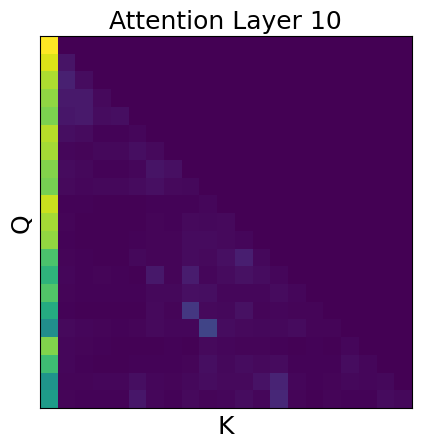
\includegraphics[width=0.86\linewidth]{figures/obs4_no_intervention.png}
    \caption{No intervention}
    \label{fig:no_intervention}
  \end{subfigure}
  \begin{subfigure}[t]{0.22\textwidth}
    \centering
    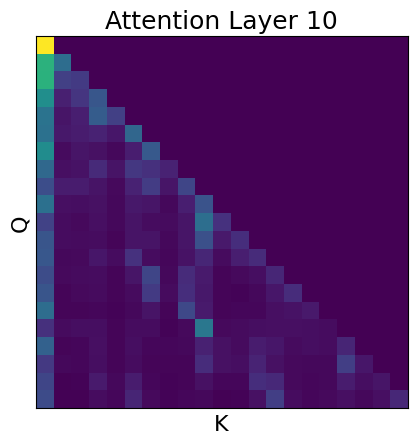
\includegraphics[width=0.86\linewidth]{figures/obs4_intervention1.png}
    \caption{nullify $b_Q$}
    \label{fig:intervention1}
  \end{subfigure}
  \begin{subfigure}[t]{0.22\textwidth}
    \centering
    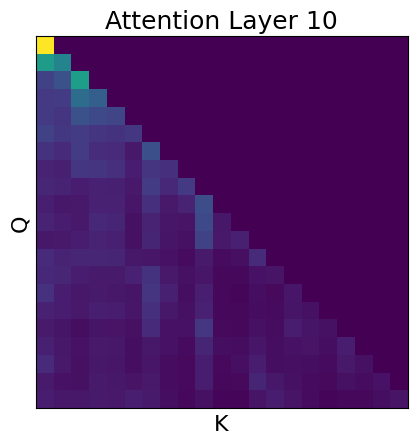
\includegraphics[width=0.86\linewidth]{figures/obs4_intervention2.png}
    \caption{remove first EPE}
    \label{fig:intervention2}
  \end{subfigure}
  \begin{subfigure}[t]{0.22\textwidth}
    \centering
    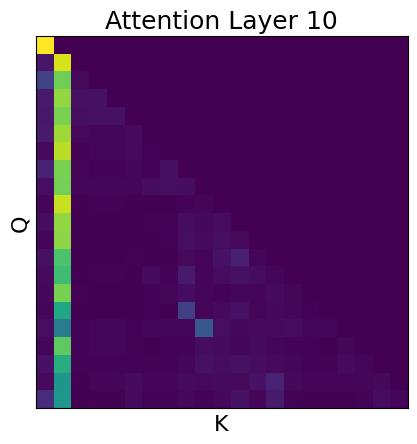
\includegraphics[width=0.86\linewidth]{figures/obs4_intervention3.png}
    \caption{move first EPE}
    \label{fig:intervention3}
  \end{subfigure}


  % ---- Bottom row (3 subfigures, with explicit horizontal gap) ----
  % Set the adjustable spacing between bottom subfigures:
  \newcommand{\bottomsep}{0.02\textwidth} % <- adjust this number to control spacing

  \begin{subfigure}[t]{0.22\textwidth}
    \centering
    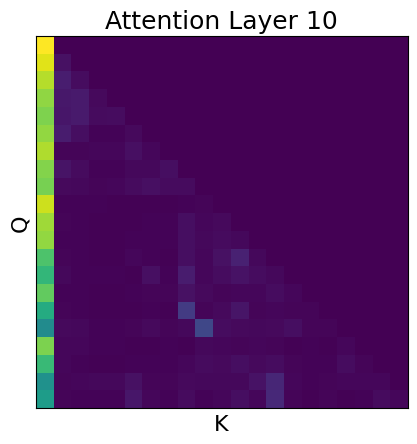
\includegraphics[width=0.86\linewidth]{figures/obs4_intervention4.png}
    \caption{nullify BOS}
    \label{fig:intervention4}
  \end{subfigure}\hspace{\bottomsep}
  \begin{subfigure}[t]{0.22\textwidth}
    \centering
    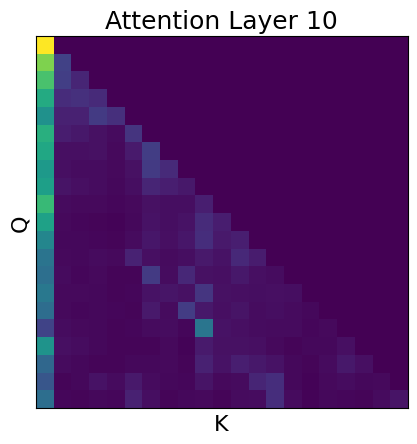
\includegraphics[width=0.86\linewidth]{figures/obs4_intervention5.png}
    \caption{nullify massive activation rows of $W_k$}
    \label{fig:intervention5}
  \end{subfigure}\hspace{\bottomsep}
  \begin{subfigure}[t]{0.22\textwidth}
    \centering
    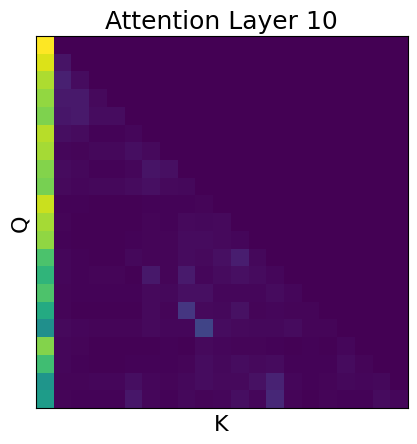
\includegraphics[width=0.86\linewidth]{figures/obs4_intervention5_2.png}
    \caption{nullify random rows of $W_k$}
    \label{fig:intervention5_2}
  \end{subfigure}


  \caption{Comparison of attention maps under different interventions. (a) no intervention; (b) intervention 1: nullify $b_Q$; (c) intervention 2: remove the learned EPE at position 1 and add a different EPE (the second); (d) intervention 3: transplant the learned EPE to another position (the second). (e) intervention 4: nullify BOS token embedding. (f) intervention 5: nullify massive activation rows of Wk. (g) nullify random rows of Wk.}
  \label{fig:interventions_comparison}
\end{figure*}


\subsubsection{Causal Interventions}
\label{sec:interventions}
To establish causality beyond correlation, we perform targeted 
interventions on each mechanism component during forward passes to test necessity (removing a component) and sufficiency (transplanting it) of each component. Full intervention results across all layers are provided in Appendix \ref{app:interventions}.



\begin{itemize}[leftmargin=*]
  \item \textbf{Intervention 1 — Nullify $b_Q$ (query bias is necessary).} Set $b_Q$ to zero; the sink substantially diminishes (\cref{fig:intervention1}), showing that $b_Q$ is necessary for the large first-token contribution.
  \item \textbf{Intervention 2 — Replace $\mathrm{EPE}_1$ (specificity of the positional signal).} Swap $\mathrm{EPE}_1$ with another position’s EPE; the first-position sink disappears (\cref{fig:intervention2}), indicating that $\mathrm{EPE}_1$ is critical to induce a sink.
  \item \textbf{Intervention 3 — Moving $\mathrm{EPE}_1$ induces a sink at the new token (sufficiency).} We transplant $\mathrm{EPE}_1$ from position 1 to position 2 (and give position 1 a different EPE). A strong sink forms at position 2 (\cref{fig:intervention3}), demonstrating that $\mathrm{EPE}_1$ is sufficient to elicit a sink at the new location.
  \item \textbf{Intervention 4 — BOS token does not drive the sink.} We zero the BOS token embedding before adding positional signals. The sink persists (\cref{fig:intervention4}), ruling out the embedding of the BOS token as a main driver of the sink.
  \item \textbf{Intervention 5 — Zero $W_k$ at bias-projection coordinates (structural pathway is necessary).} Zero $W_k$ rows at massive-$\mathrm{EPE}_1$ coordinates compared to zeroing $W_k$ rows at random coordinates; only the prior case substantially reduces the sink (\cref{fig:intervention5}, \cref{fig:intervention5_2}), confirming that these specific coordinates are core drivers for translating $\mathrm{EPE}_1$ into the attention bias.
\end{itemize}

\section{Conclusions}
Attention sinks are robust across Transformer architectures and modalities, but mechanisms differ by architecture. In GPT-2–style models, we identify a concrete implementation pathway: interaction between  (i) a learned query bias, (ii) the 
first-layer transformation of positional information, and (iii) structure 
in the key projection. Crucially, this circuit cannot account for sinks in architectures lacking these components—models without learned query biases or that use alternative positional schemes (ALiBi, or no positional encodings)—yet these also exhibit attention sinks. This implies that while attention sinks are robust as a phenomenon, they are not governed by a single universal mechanism.

\paragraph{Implications}
The lack of a single universal mechanism reveals attention sinks as an optimization-friendly attractor: when multiple pathways exist, training reliably discovers circuits that implement the sink behavior. This has important implications for both understanding and controlling these phenomena. First, it suggests that attention sinks may serve a fundamental computational role that emerges regardless of specific architectural choices. Second, it indicates that effective mitigation strategies must be mechanism-aware. Naive interventions targeting individual components will likely fail, as optimization can compensate through alternative pathways. Instead, successful approaches must either address the underlying computational pressures that drive sink formation, or develop architecture-specific interventions. 



\section{Limitations}

\subsection{Scope across architectures and scales}
Our analyses focus on a GPT-2–style model with learned query biases and absolute positional encodings. The broader Transformer ecosystem includes architectures that omit such biases or use alternative positional schemes (e.g., RoPE, ALiBi). While we do show that the same circuit can not form in those settings, we leave the investigation of specific mechanisms that do form in these models to future work. In addition, GPT-2 is small by contemporary standards; with scale, the mechanism could strengthen, fragment into multiple pathways, or be replaced by different circuits.

\subsection{Learning dynamics}
We provide a post-hoc, static analysis of a trained checkpoint. We do not track when the circuit emerges during pre-training, which gradients give rise to it, or whether intermediate snapshots exhibit qualitatively different pathways. We believe our static analysis could inform future work researching the emergence of the attention sink mechanism.

\subsection{Mechanism vs. function}
Our contribution is mechanistic: we explain \emph{how} an attention sink can be implemented in the studied architecture. We do not claim a definitive functional rationale for \emph{why} such a sink is beneficial or harmful across tasks. Establishing the downstream utility or cost of the sink, and the conditions under which it is selected by optimization, is left for future work.

\bibliography{custom}

\appendix

\section{Further Experiments}

\subsection{Effective positional encoding demonstration} \label{app:epe_exp}
In this section, we illustrate that $\mathrm{EPE}_i$ roughly captures the net positional signal that is added to the input after the first layer's transformation when adding the positional encoding $p_i$ to the input $x_i^{(0)}$. To that end, we define an approximation of the result of processing the input by the first MLP: $R_i \coloneq x_i^{(0)} + MLP^{(1)}(x_i^{(0)})$. We then define the input without positional information $e_i \coloneq x_i^{(0)}-p_i$, and the result of processing the input without the positional information: $O_i=e_i + MLP^{(1)}(e_i)$. We then compare \(\mathrm{EPE}_i\) to the difference \(R_i - O_i\), computing the cosine similarity for each token \(i\). This directly measures whether the incremental contribution caused by adding \(p_i\) aligns in direction with \(\mathrm{EPE}_i\). The results range between $0.776$ at the lowest and $0.996$ at the highest (\cref{fig:epe_exp}). These similarities are very high, indicating that $\mathrm{EPE}_i$ represents the effective contribution of positional information after being processed through the network's initial transformations.

\begin{figure}[t]
  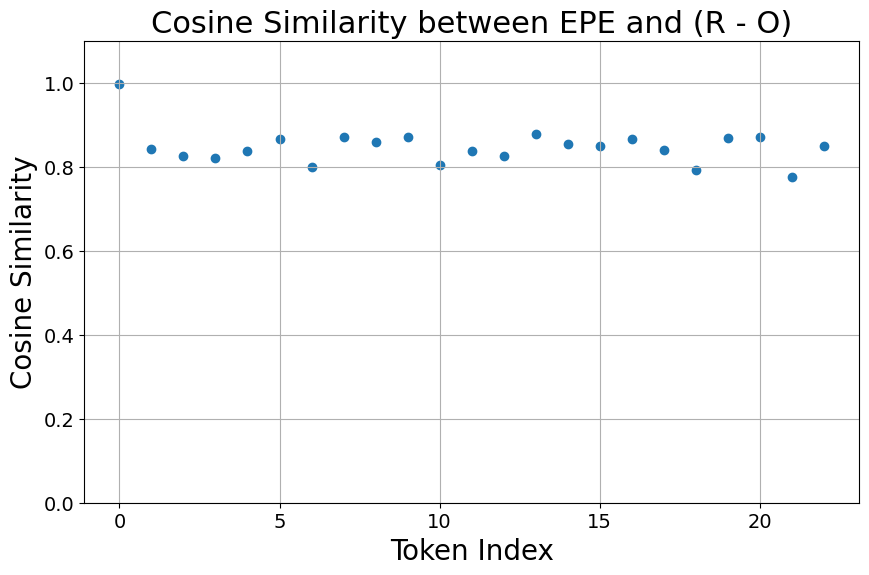
\includegraphics[width=\columnwidth]{figures/epe_exp.png}
  \caption{Coordinate values of $\mathrm{EPE}_i$ for the first token (replicating the distribution described in \cref{sec:wk_structure}). Most coordinates are near zero; a small set exhibits extremely large magnitudes (``massive activations'').}
  \label{fig:epe_exp}
\end{figure}

\subsection{Bias Term Magnitude Across All Layers}\label{app:bias_term}

This section reproduces the bias-term magnitude analysis from \cref{sec:delta_analysis} across all layers: we plot the distribution of $\Delta_j^{(i)} \triangleq b_Q^{(i)}W_k^{(i)\top} x_j^{(i)\top}$, across positions for each layer (cf. \cref{fig:obs1_layer10}). In most layers, the first-position term $\Delta_1^{(i)}$ is a conspicuous outlier, indicating a strong prior to attend to position 1 (see \cref{fig:appendix_obs1_all_layers}).

\begin{figure*}[t]
  \begin{subfigure}[t]{0.24\textwidth}
    \centering
    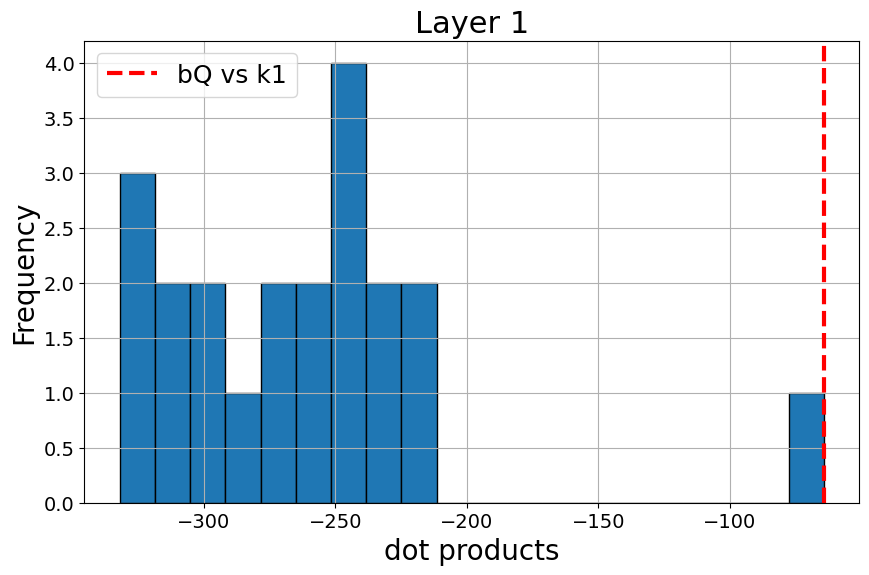
\includegraphics[width=1.4\columnwidth]{figures/obs1_appendix/obs1_layer1.png}
    \caption{layer 1}
  \end{subfigure}\hfill
  \begin{subfigure}[t]{0.24\textwidth}
    \centering
    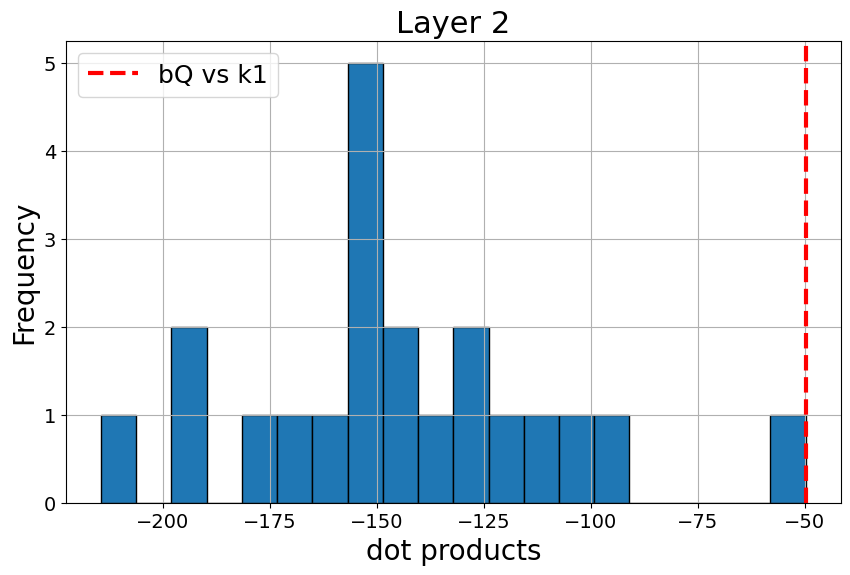
\includegraphics[width=1.4\columnwidth]{figures/obs1_appendix/obs1_layer2.png}
    \caption{layer 2}
  \end{subfigure}\hfill
  \begin{subfigure}[t]{0.24\textwidth}
    \centering
    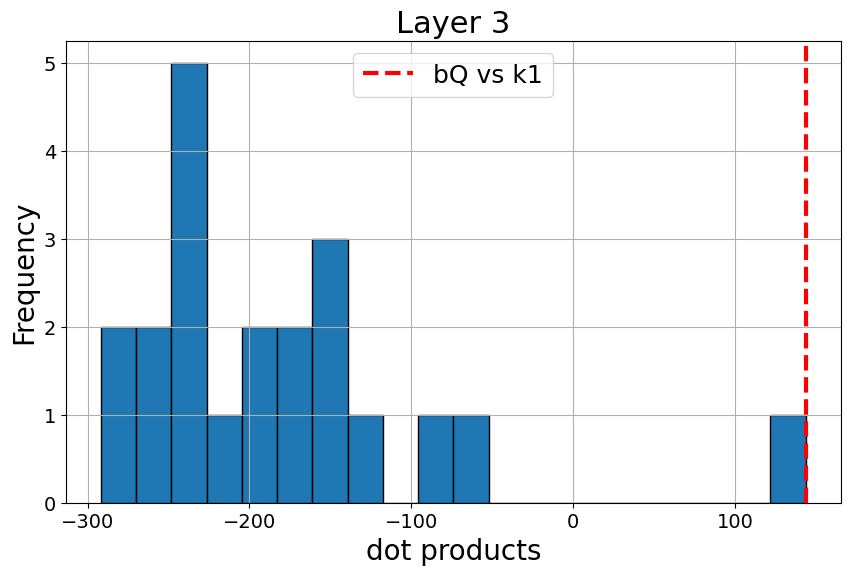
\includegraphics[width=1.4\columnwidth]{figures/obs1_appendix/obs1_layer3.png}
    \caption{layer 3}
  \end{subfigure}\hfill
    \vspace{2mm}

  \begin{subfigure}[t]{0.24\textwidth}
    \centering
    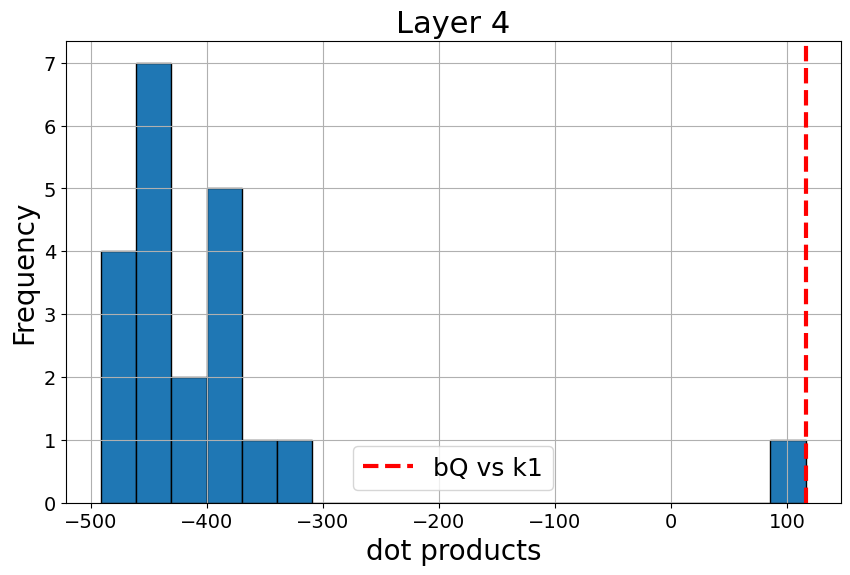
\includegraphics[width=1.4\columnwidth]{figures/obs1_appendix/obs1_layer4.png}
    \caption{layer 4}
  \end{subfigure}\hfill
  \begin{subfigure}[t]{0.24\textwidth}
    \centering
    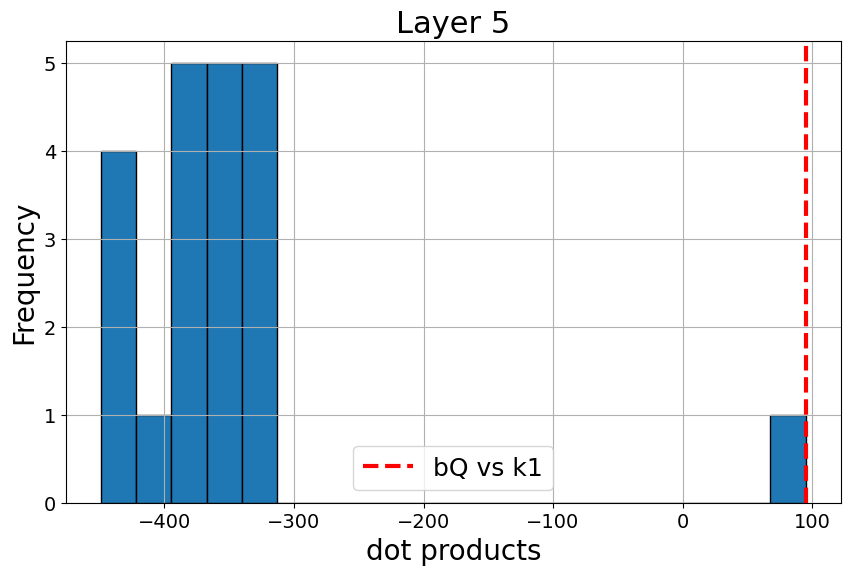
\includegraphics[width=1.4\columnwidth]{figures/obs1_appendix/obs1_layer5.png}
    \caption{layer 5}
  \end{subfigure}\hfill
  \begin{subfigure}[t]{0.24\textwidth}
    \centering
    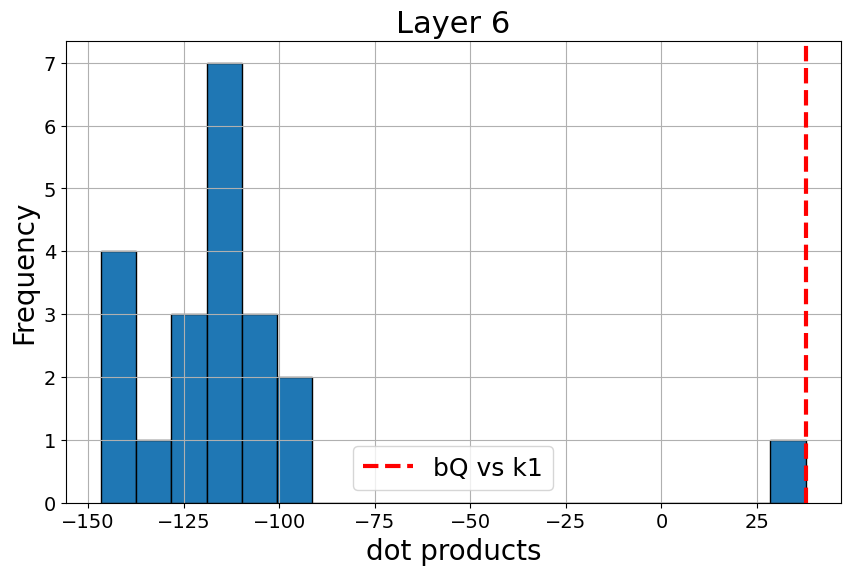
\includegraphics[width=1.4\columnwidth]{figures/obs1_appendix/obs1_layer6.png}
    \caption{layer 6}
  \end{subfigure}\hfill
    \vspace{2mm}

    \begin{subfigure}[t]{0.24\textwidth}
    \centering
    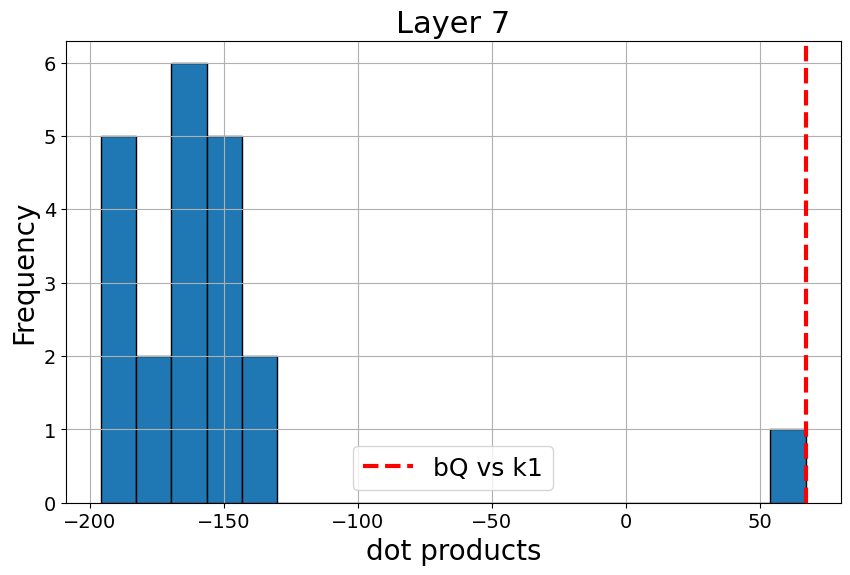
\includegraphics[width=1.4\columnwidth]{figures/obs1_appendix/obs1_layer7.png}
    \caption{layer 7}
  \end{subfigure}\hfill
      \begin{subfigure}[t]{0.24\textwidth}
    \centering
    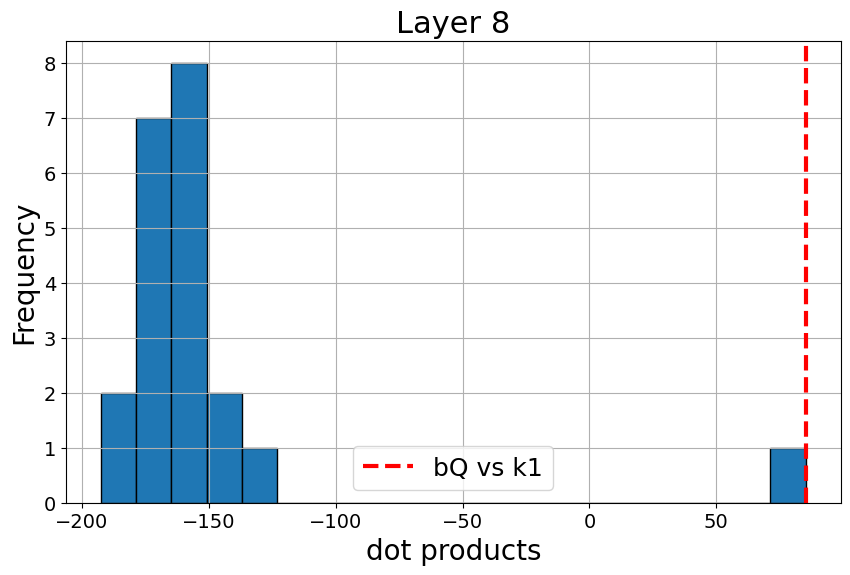
\includegraphics[width=1.4\columnwidth]{figures/obs1_appendix/obs1_layer8.png}
    \caption{layer 8}
  \end{subfigure}\hfill
      \begin{subfigure}[t]{0.24\textwidth}
    \centering
    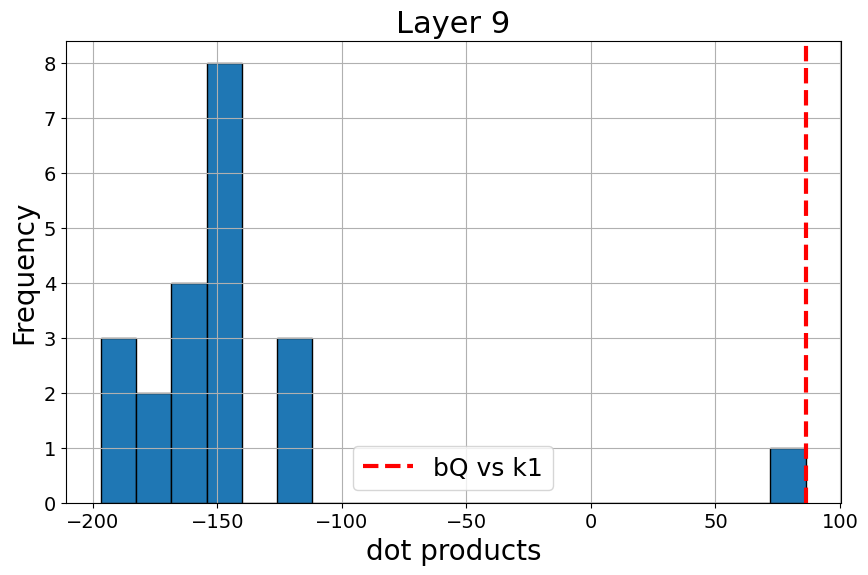
\includegraphics[width=1.4\columnwidth]{figures/obs1_appendix/obs1_layer9.png}
    \caption{layer 9}
  \end{subfigure}\hfill
    \vspace{2mm}
    
    \begin{subfigure}[t]{0.24\textwidth}
    \centering
    \includegraphics[width=1.4\columnwidth]{figures/obs1_appendix/obs1_layer10.png}
    \caption{layer 10}
  \end{subfigure}\hfill
    \begin{subfigure}[t]{0.24\textwidth}
    \centering
    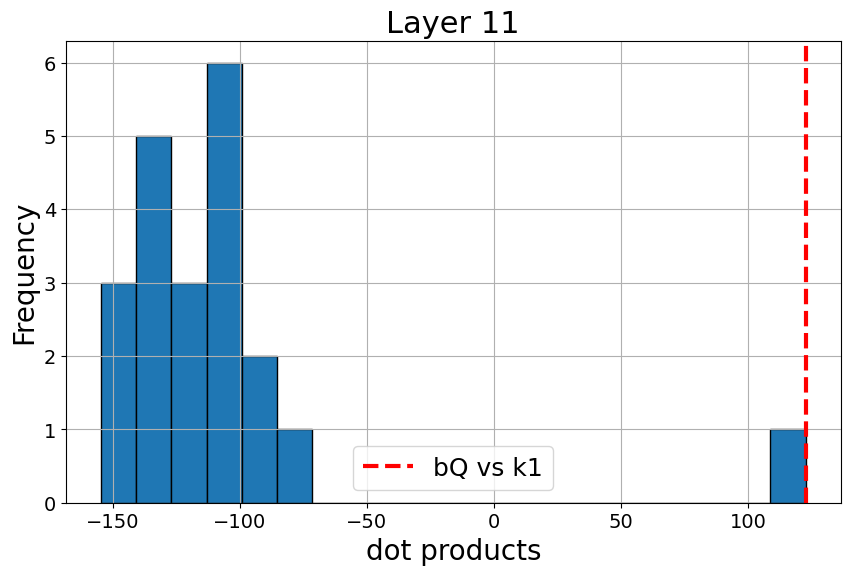
\includegraphics[width=1.4\columnwidth]{figures/obs1_appendix/obs1_layer11.png}
    \caption{layer 11}
  \end{subfigure}\hfill
  \begin{subfigure}[t]{0.24\textwidth}
    \centering
    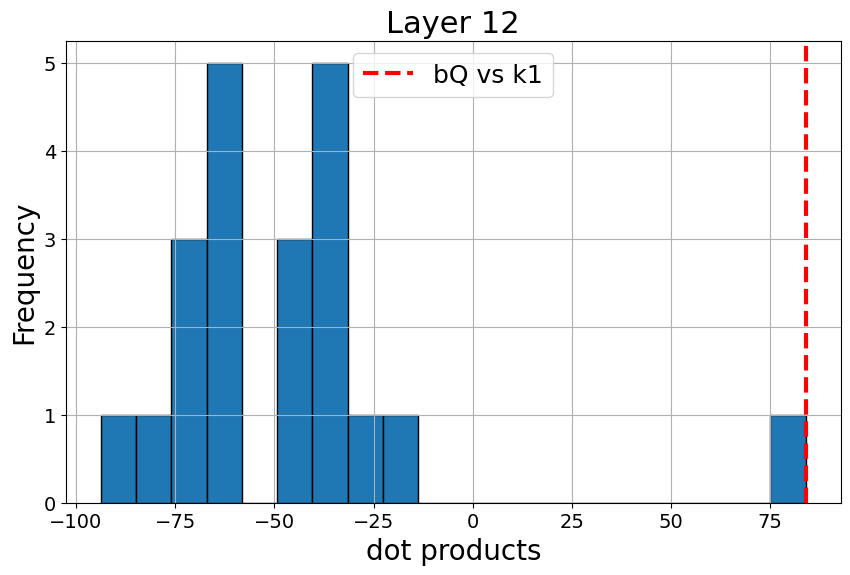
\includegraphics[width=1.4\columnwidth]{figures/obs1_appendix/obs1_layer12.png}
    \caption{layer 12}
  \end{subfigure}\hfill
  \vspace{2mm}
  \caption{Bias-term distributions $\Delta_j$ across positions $j$ for each layer $i$ (replicating \cref{fig:obs1_layer10}). Red denotes the first-position term $\Delta_1^{(i)}$; blue denotes all other positions. In most layers, the red distribution is shifted far to the right, evidencing an anomalously large first-position bias.}
  \label{fig:appendix_obs1_all_layers}
\end{figure*}

\subsection{EPE-Bias Alignment Across All Layers}\label{app:epe_bias}

This section repeats the alignment analysis from \cref{sec:epe_alignment}: for each layer $i$ and position $j$ we compute $\cos\big(b_Q^{(i)},\, \mathrm{EPE}_jW_k^{(i)}\big)$, highlighting position 1. In most layers, position 1 shows strong positive alignment while other positions do not (see \cref{fig:appendix_obs2_all_layers}).

\begin{figure*}[t]
  \begin{subfigure}[t]{0.24\textwidth}
    \centering
    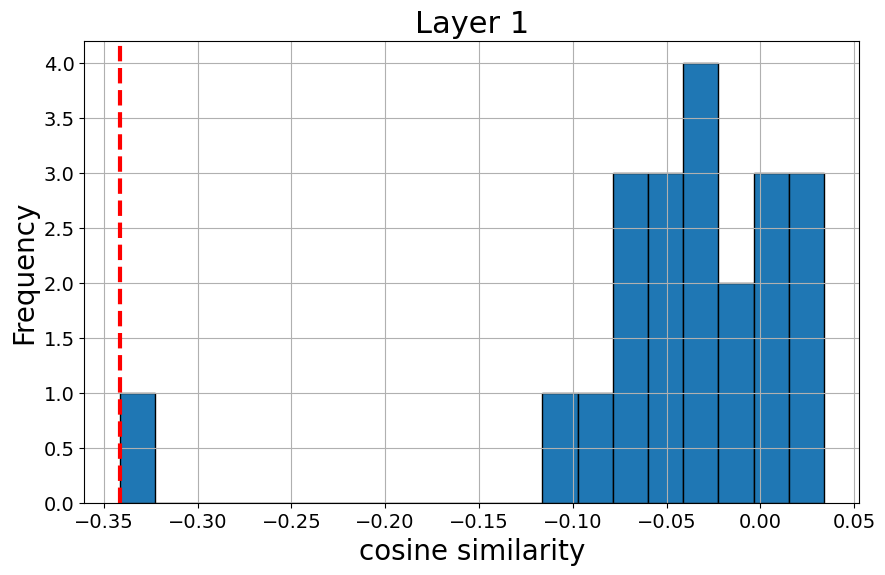
\includegraphics[width=1.4\columnwidth]{figures/obs2_appendix/obs2_layer1.png}
    \caption{layer 1}
  \end{subfigure}\hfill
  \begin{subfigure}[t]{0.24\textwidth}
    \centering
    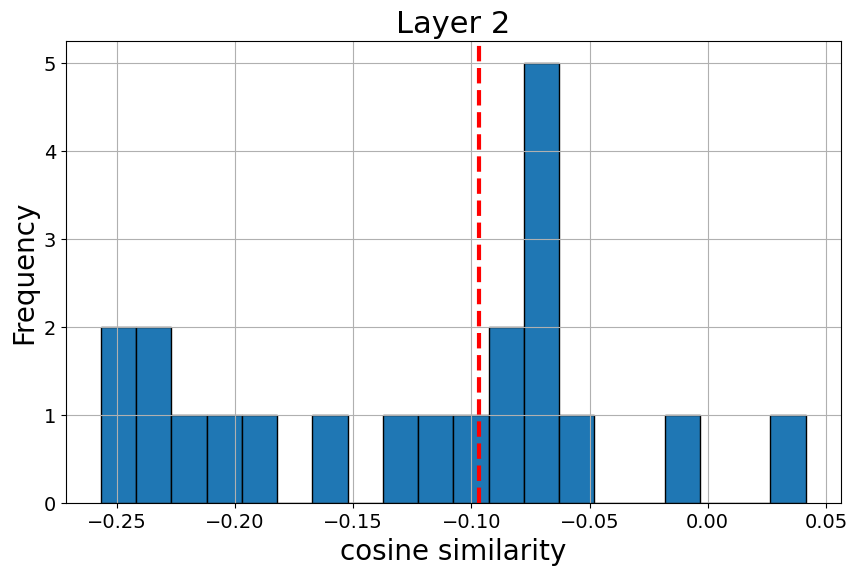
\includegraphics[width=1.4\columnwidth]{figures/obs2_appendix/obs2_layer2.png}
    \caption{layer 2}
  \end{subfigure}\hfill
  \begin{subfigure}[t]{0.24\textwidth}
    \centering
    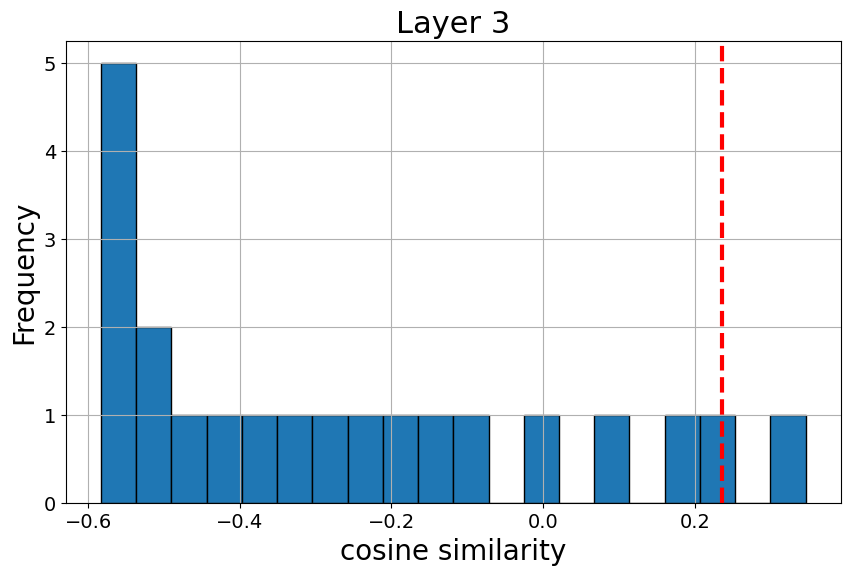
\includegraphics[width=1.4\columnwidth]{figures/obs2_appendix/obs2_layer3.png}
    \caption{layer 3}
  \end{subfigure}\hfill
    \vspace{2mm}

  \begin{subfigure}[t]{0.24\textwidth}
    \centering
    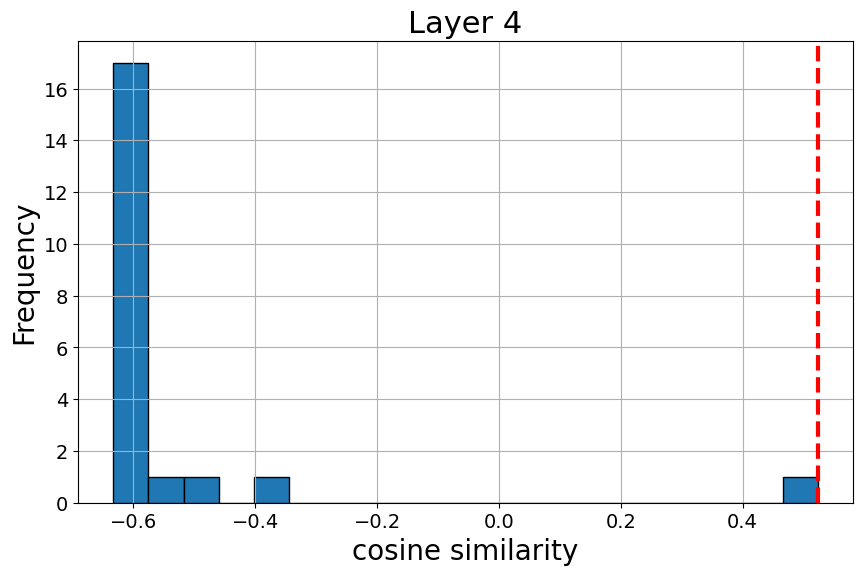
\includegraphics[width=1.4\columnwidth]{figures/obs2_appendix/obs2_layer4.png}
    \caption{layer 4}
  \end{subfigure}\hfill
  \begin{subfigure}[t]{0.24\textwidth}
    \centering
    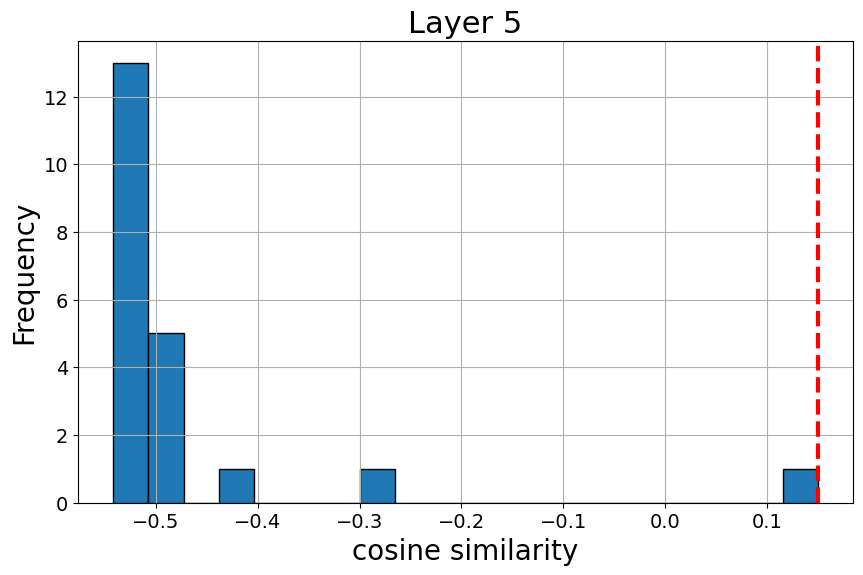
\includegraphics[width=1.4\columnwidth]{figures/obs2_appendix/obs2_layer5.png}
    \caption{layer 5}
  \end{subfigure}\hfill
  \begin{subfigure}[t]{0.24\textwidth}
    \centering
    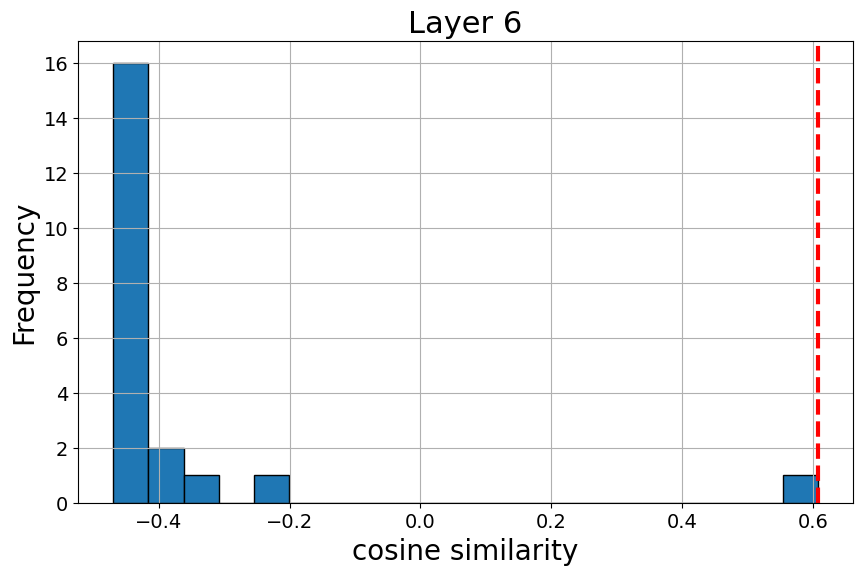
\includegraphics[width=1.4\columnwidth]{figures/obs2_appendix/obs2_layer6.png}
    \caption{layer 6}
  \end{subfigure}\hfill
    \vspace{2mm}

    \begin{subfigure}[t]{0.24\textwidth}
    \centering
    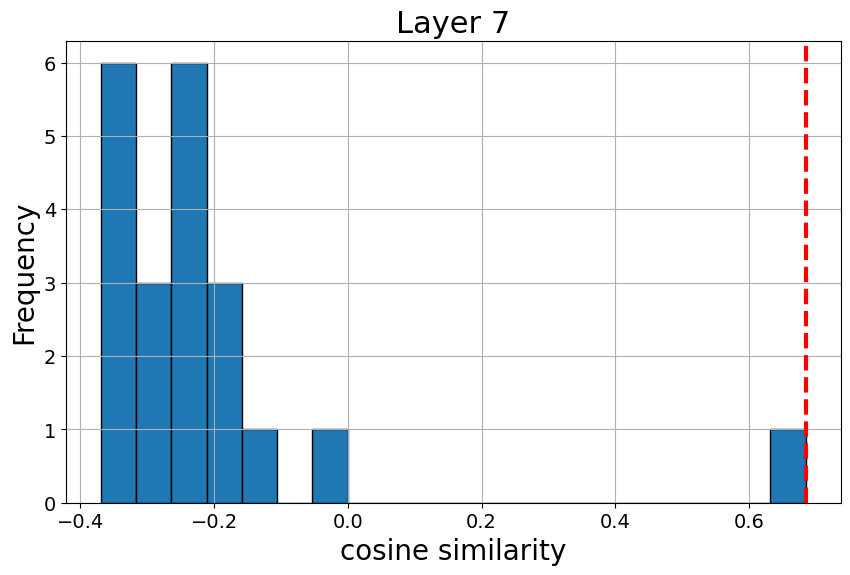
\includegraphics[width=1.4\columnwidth]{figures/obs2_appendix/obs2_layer7.png}
    \caption{layer 7}
  \end{subfigure}\hfill
      \begin{subfigure}[t]{0.24\textwidth}
    \centering
    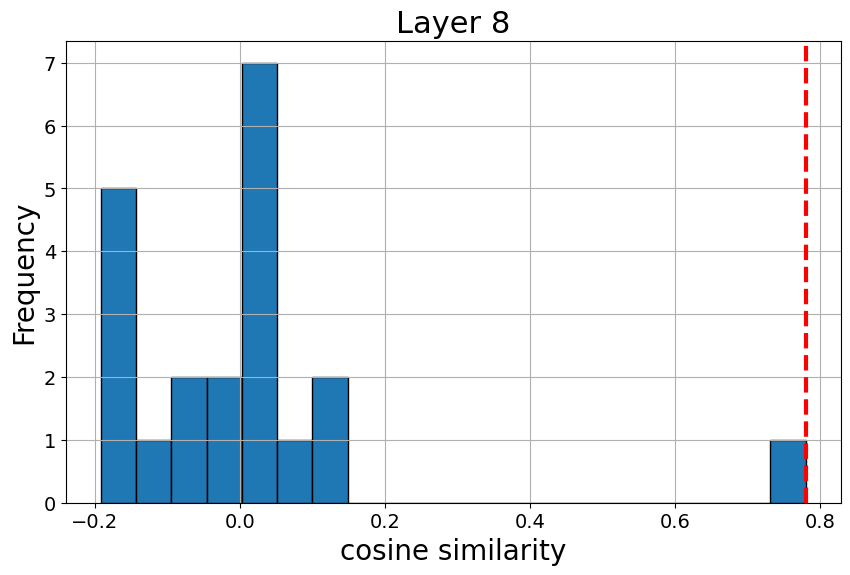
\includegraphics[width=1.4\columnwidth]{figures/obs2_appendix/obs2_layer8.png}
    \caption{layer 8}
  \end{subfigure}\hfill
      \begin{subfigure}[t]{0.24\textwidth}
    \centering
    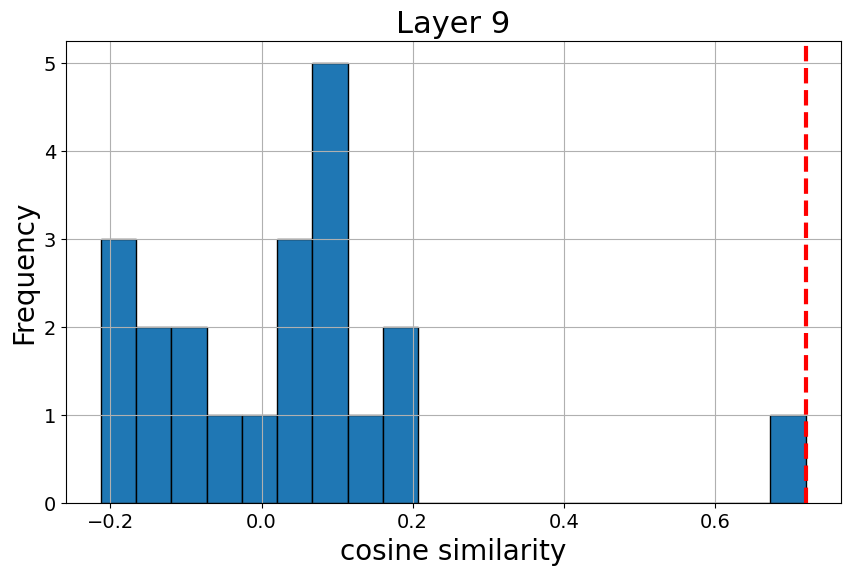
\includegraphics[width=1.4\columnwidth]{figures/obs2_appendix/obs2_layer9.png}
    \caption{layer 9}
  \end{subfigure}\hfill
    \vspace{2mm}
    
    \begin{subfigure}[t]{0.24\textwidth}
    \centering
    \includegraphics[width=1.4\columnwidth]{figures/obs2_appendix/obs2_layer10.png}
    \caption{layer 10}
  \end{subfigure}\hfill
    \begin{subfigure}[t]{0.24\textwidth}
    \centering
    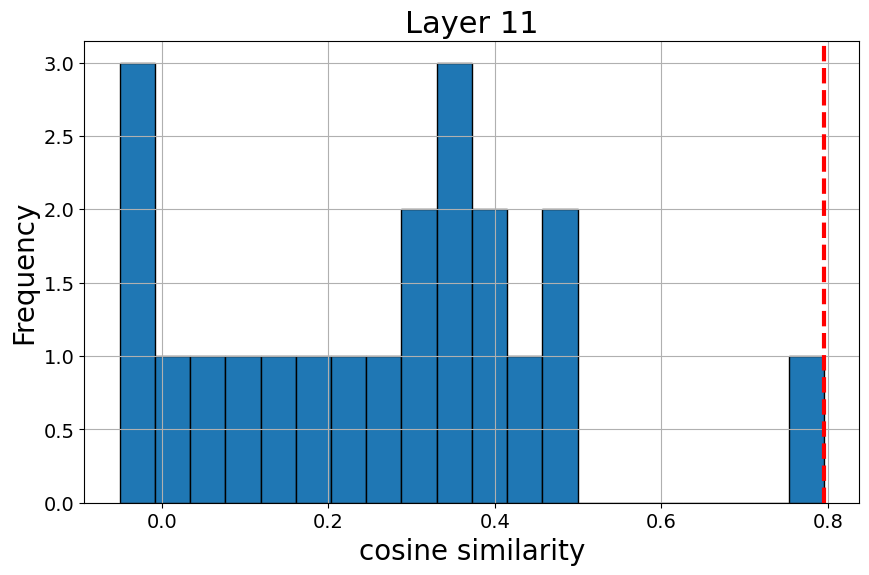
\includegraphics[width=1.4\columnwidth]{figures/obs2_appendix/obs2_layer11.png}
    \caption{layer 11}
  \end{subfigure}\hfill
  \begin{subfigure}[t]{0.24\textwidth}
    \centering
    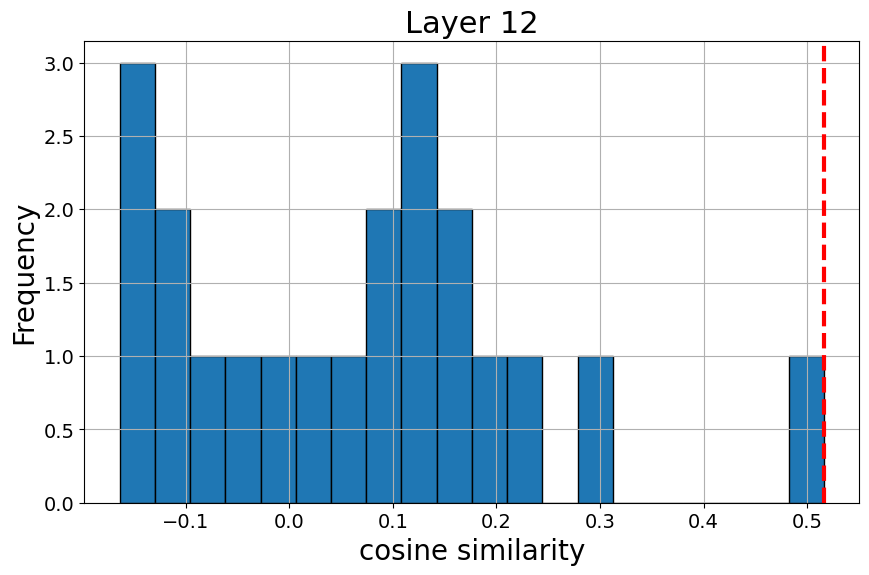
\includegraphics[width=1.4\columnwidth]{figures/obs2_appendix/obs2_layer12.png}
    \caption{layer 12}
  \end{subfigure}\hfill
    \vspace{2mm}

  \caption{Cosine similarity between the query bias and EPE-projected keys across layers and positions (replicating \cref{fig:obs2_layer10}). For each layer $i$ and position $j$, we plot $\cos\big(b_Q^{(i)},\, \mathrm{EPE}_jW_k^{(i)}\big)$. Red marks position $j{=}1$; blue marks all other positions. Position 1 shows strong positive alignment while other positions do not, indicating that $\mathrm{EPE}_1W_k^{(i)}$ is specifically aligned with $b_Q^{(i)}$.}
  \label{fig:appendix_obs2_all_layers}
\end{figure*}

\subsection{Identifying Massive Activations in First-Position EPE}\label{app:massive_activations_in_ppe}

This section explains how we identify coordinates with unusually large absolute values in $\mathrm{EPE}_1$. We select coordinates whose absolute values exceed the mean absolute value by at least three standard deviations; in our model this criterion selects indices 105, 218, and 329. Elements at these indices are clear outliers, each more than 15 standard deviations away from the mean. Each such selected dimension exhibits the coordinate-level phenomenon described in \cref{sec:wk_structure} (i.e., large $|\gamma^{(i)}[d]|$ and a strong contribution to the source-agnostic shift). See \cref{fig:appendix_massive_activations} for a visualization of $\mathrm{EPE}_1$. It is clear visually that coordinates 105, 218, and 329 have conspicuously larger norms than other indices. 

\begin{figure}[t]
  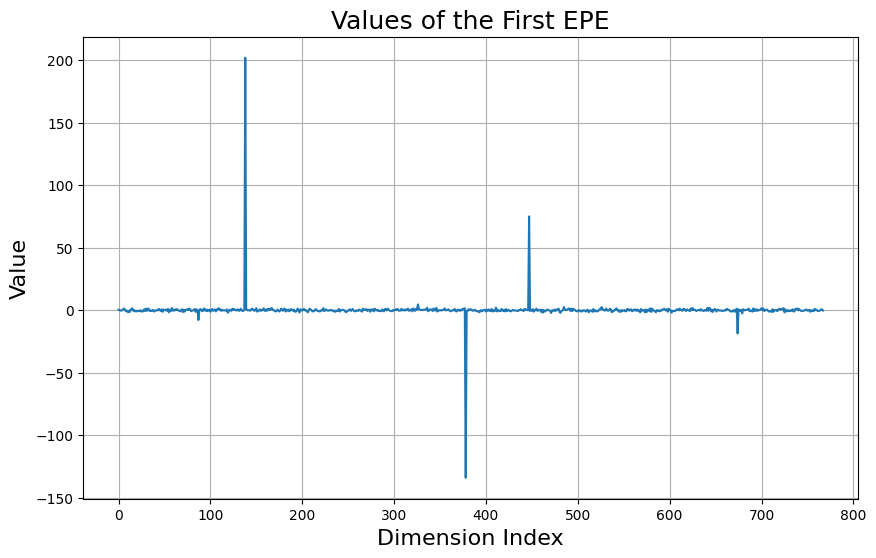
\includegraphics[width=\columnwidth]{figures/massive_activations_in_ppe.png}
  \caption{Coordinate values of $\mathrm{EPE}_1$ for the first token (replicating the distribution described in \cref{sec:wk_structure}). Most coordinates are near zero; a small set exhibits extremely large magnitudes (``massive activations'').}
  \label{fig:appendix_massive_activations}
\end{figure}

\subsection{Coordinate-Level Alignment Across All Layers} \label{app:coor_align}

This section tabulates $\gamma^{(i)}=b_Q^{(i)}W_k^{(i)\top}$ at coordinates where $|\mathrm{EPE}_1|$ is conspicuously large, mirroring the coordinate-level analysis in \cref{sec:wk_structure}. Values are compared against the baseline mean $\pm$ two standard deviations across all coordinates (see \cref{tab:appendix_coor_align}).

\begin{table}[t]
  \centering
  \begin{tabular}{llll}
    \hline
    \textbf{Layer} & \textbf{Baseline} & \textbf{$d{=}138$} & \textbf{$d{=}447$}\\
    \hline
    layer 1   &   4.47$\pm$22.226 &  12.116   &    11.064        \\
    layer 2   &   2.8$\pm$6.62    &    8.065   &    24.468         \\
    layer 3   &   1.717$\pm$5.826 &    10.178  &    23.047        \\
    layer 4   &   1.657$\pm$5.02  &   18.199   &     17.149         \\
    layer 5   &   1.561$\pm$4.618 &    3.072   &    23.854          \\
    layer 6   &   0.86$\pm$1.59   &    5.644   &    6.142          \\
    layer 8   &   1.404$\pm$3.546 &    19.806  &    28.01          \\
    layer 10  &   1.313$\pm$3.618 &    23.131  &    28.42        \\
    layer 12   &   1.145$\pm$2.65 &    4.5  &    13.59         \\

    \hline
  \end{tabular}
  \caption{$\gamma^{(i)}=b_Q^{(i)}W_k^{(i)\top}$ at coordinates where $\mathrm{EPE}_1$ has massive activations (dims 138, 447) versus the baseline mean $\pm$ two standard deviations across all coordinates. Massive-$\mathrm{EPE}_1$ coordinates consistently exceed the baseline, indicating that $\mathrm{EPE}_1$ is irregularly large precisely where the bias projection is large.}
  \label{tab:appendix_coor_align}
\end{table}

\subsection{Intervention Results Across All Layers}\label{app:interventions}

This section reproduces the intervention analyses from \cref{sec:interventions} across all layers, including the baseline and five targeted interventions. Each subsection mirrors the corresponding main-text figure and shows the layer-wise attention maps.

\subsubsection{Baseline: No Intervention}\label{app:no_intervention}

We show attention maps with no intervention (cf. \cref{fig:no_intervention}), demonstrating the prevalence of the first-position sink across layers (see \cref{fig:app_no_intervention_all_layers}).
\begin{figure*}[t]
  \begin{subfigure}[t]{0.24\textwidth}
    \centering
    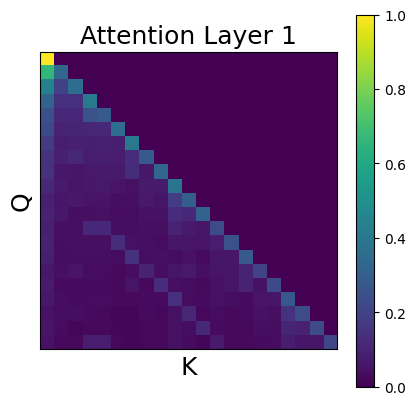
\includegraphics[width=1.4\columnwidth]{figures/no_intervention/layer_1.png}
    \caption{layer 1}
  \end{subfigure}\hfill
  \begin{subfigure}[t]{0.24\textwidth}
    \centering
    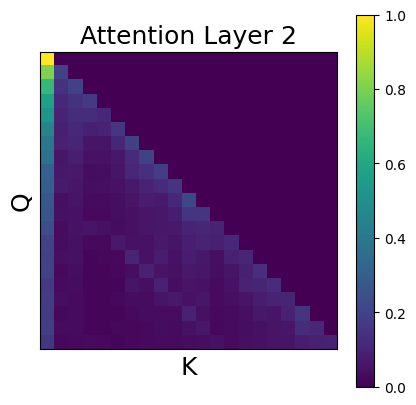
\includegraphics[width=1.4\columnwidth]{figures/no_intervention/layer_2.png}
    \caption{layer 2}
  \end{subfigure}\hfill
  \begin{subfigure}[t]{0.24\textwidth}
    \centering
    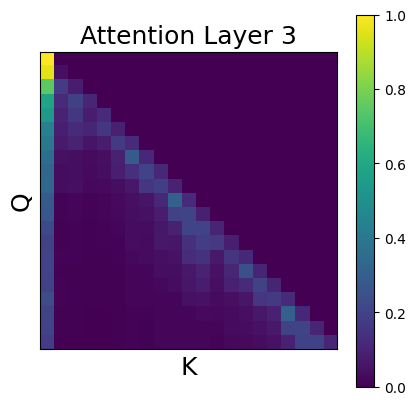
\includegraphics[width=1.4\columnwidth]{figures/no_intervention/layer_3.png}
    \caption{layer 3}
  \end{subfigure}\hfill

  \begin{subfigure}[t]{0.24\textwidth}
    \centering
    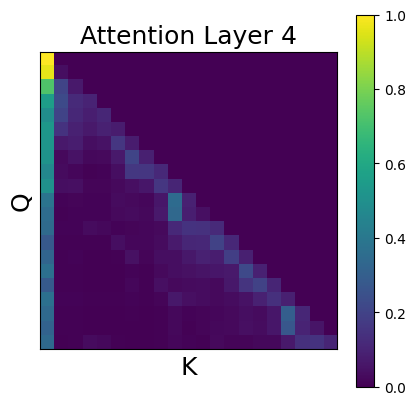
\includegraphics[width=1.4\columnwidth]{figures/no_intervention/layer_4.png}
    \caption{layer 4}
  \end{subfigure}\hfill
  \begin{subfigure}[t]{0.24\textwidth}
    \centering
    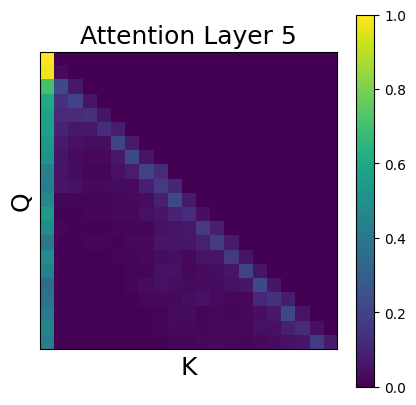
\includegraphics[width=1.4\columnwidth]{figures/no_intervention/layer_5.png}
    \caption{layer 5}
  \end{subfigure}\hfill
  \begin{subfigure}[t]{0.24\textwidth}
    \centering
    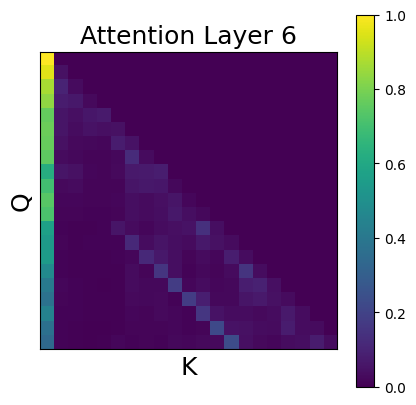
\includegraphics[width=1.4\columnwidth]{figures/no_intervention/layer_6.png}
    \caption{layer 6}
  \end{subfigure}\hfill

    \begin{subfigure}[t]{0.24\textwidth}
    \centering
    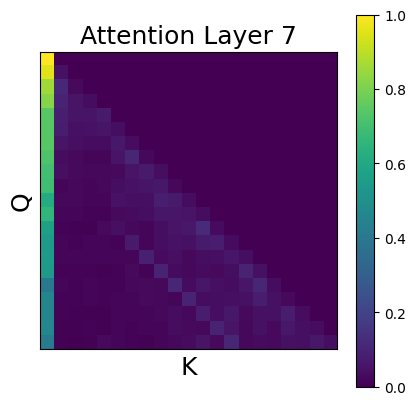
\includegraphics[width=1.4\columnwidth]{figures/no_intervention/layer_7.png}
    \caption{layer 7}
  \end{subfigure}\hfill
      \begin{subfigure}[t]{0.24\textwidth}
    \centering
    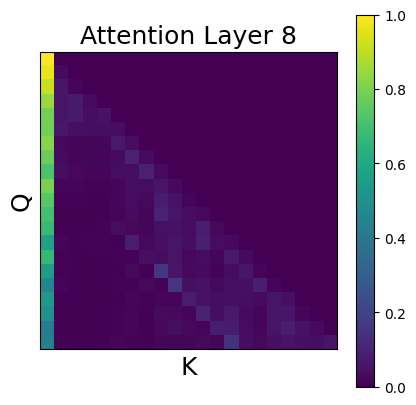
\includegraphics[width=1.4\columnwidth]{figures/no_intervention/layer_8.png}
    \caption{layer 8}
  \end{subfigure}\hfill
      \begin{subfigure}[t]{0.24\textwidth}
    \centering
    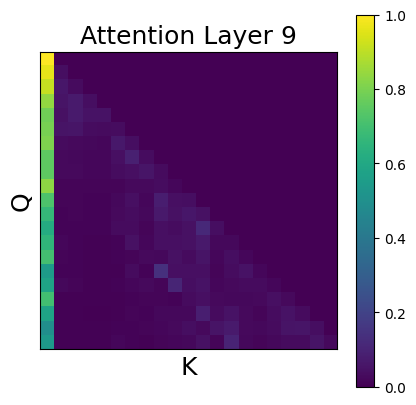
\includegraphics[width=1.4\columnwidth]{figures/no_intervention/layer_9.png}
    \caption{layer 9}
  \end{subfigure}\hfill
    
    \begin{subfigure}[t]{0.24\textwidth}
    \centering
    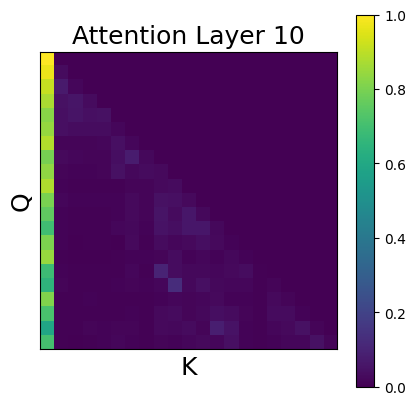
\includegraphics[width=1.4\columnwidth]{figures/no_intervention/layer_10.png}
    \caption{layer 10}
  \end{subfigure}\hfill
    \begin{subfigure}[t]{0.24\textwidth}
    \centering
    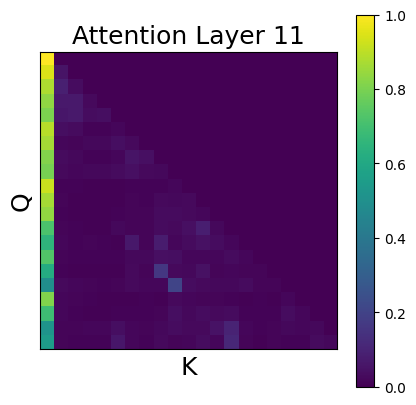
\includegraphics[width=1.4\columnwidth]{figures/no_intervention/layer_11.png}
    \caption{layer 11}
  \end{subfigure}\hfill
  \begin{subfigure}[t]{0.24\textwidth}
    \centering
    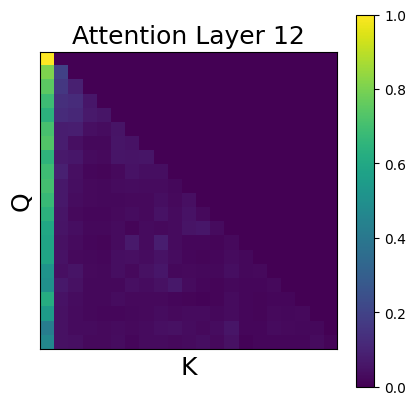
\includegraphics[width=1.4\columnwidth]{figures/no_intervention/layer_12.png}
    \caption{layer 12}
  \end{subfigure}\hfill

  \caption{Attention maps for all layers with no intervention (replicating \cref{fig:no_intervention}). A prominent first-position sink is visible in most layers.}
  \label{fig:app_no_intervention_all_layers}
\end{figure*}


\subsubsection{Intervention 1: Nullifying Query Bias}\label{app:intervention1}

We zero $b_Q$ (cf. \cref{fig:intervention1}), which substantially diminishes the sink across layers.
\begin{figure*}[t]
  \begin{subfigure}[t]{0.24\textwidth}
    \centering
    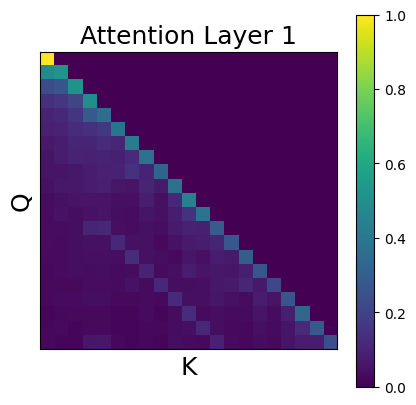
\includegraphics[width=1.4\columnwidth]{figures/intervention1/layer_1.png}
    \caption{layer 1}
  \end{subfigure}\hfill
  \begin{subfigure}[t]{0.24\textwidth}
    \centering
    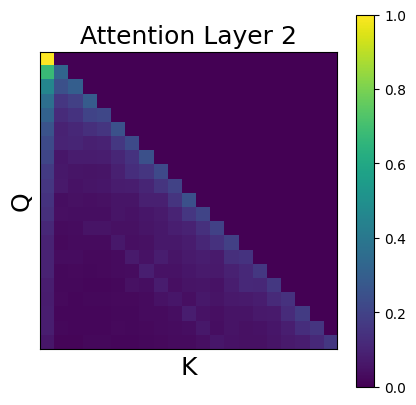
\includegraphics[width=1.4\columnwidth]{figures/intervention1/layer_2.png}
    \caption{layer 2}
  \end{subfigure}\hfill
  \begin{subfigure}[t]{0.24\textwidth}
    \centering
    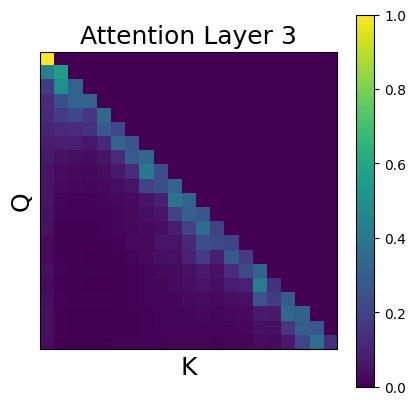
\includegraphics[width=1.4\columnwidth]{figures/intervention1/layer_3.png}
    \caption{layer 3}
  \end{subfigure}\hfill

  \begin{subfigure}[t]{0.24\textwidth}
    \centering
    \includegraphics[width=1.4\columnwidth]{figures/intervention1/layer_4.png}
    \caption{layer 4}
  \end{subfigure}\hfill
  \begin{subfigure}[t]{0.24\textwidth}
    \centering
    \includegraphics[width=1.4\columnwidth]{figures/intervention1/layer_5.png}
    \caption{layer 5}
  \end{subfigure}\hfill
  \begin{subfigure}[t]{0.24\textwidth}
    \centering
    \includegraphics[width=1.4\columnwidth]{figures/intervention1/layer_6.png}
    \caption{layer 6}
  \end{subfigure}\hfill

    \begin{subfigure}[t]{0.24\textwidth}
    \centering
    \includegraphics[width=1.4\columnwidth]{figures/intervention1/layer_7.png}
    \caption{layer 7}
  \end{subfigure}\hfill
      \begin{subfigure}[t]{0.24\textwidth}
    \centering
    \includegraphics[width=1.4\columnwidth]{figures/intervention1/layer_8.png}
    \caption{layer 8}
  \end{subfigure}\hfill
      \begin{subfigure}[t]{0.24\textwidth}
    \centering
    \includegraphics[width=1.4\columnwidth]{figures/intervention1/layer_9.png}
    \caption{layer 9}
  \end{subfigure}\hfill
    
    \begin{subfigure}[t]{0.24\textwidth}
    \centering
    \includegraphics[width=1.4\columnwidth]{figures/intervention1/layer_10.png}
    \caption{layer 10}
  \end{subfigure}\hfill
    \begin{subfigure}[t]{0.24\textwidth}
    \centering
    \includegraphics[width=1.4\columnwidth]{figures/intervention1/layer_11.png}
    \caption{layer 11}
  \end{subfigure}\hfill
  \begin{subfigure}[t]{0.24\textwidth}
    \centering
    \includegraphics[width=1.4\columnwidth]{figures/intervention1/layer_12.png}
    \caption{layer 12}
  \end{subfigure}\hfill

  \caption{Attention maps for all layers with $b_Q$ set to zero (replicating \cref{fig:intervention1}). The sink is substantially reduced across layers.}
\end{figure*}


\subsubsection{Intervention 2: Replacing First Position EPE}\label{app:intervention2}

We swap $\mathrm{EPE}_1$ with another position’s EPE (cf. \cref{fig:intervention2}), which removes the first-position sink.
\begin{figure*}[t]
  \begin{subfigure}[t]{0.24\textwidth}
    \centering
    \includegraphics[width=1.4\columnwidth]{figures/intervention2/layer_1.png}
    \caption{layer 1}
  \end{subfigure}\hfill
  \begin{subfigure}[t]{0.24\textwidth}
    \centering
    \includegraphics[width=1.4\columnwidth]{figures/intervention2/layer_2.png}
    \caption{layer 2}
  \end{subfigure}\hfill
  \begin{subfigure}[t]{0.24\textwidth}
    \centering
    \includegraphics[width=1.4\columnwidth]{figures/intervention2/layer_3.png}
    \caption{layer 3}
  \end{subfigure}\hfill

  \begin{subfigure}[t]{0.24\textwidth}
    \centering
    \includegraphics[width=1.4\columnwidth]{figures/intervention2/layer_4.png}
    \caption{layer 4}
    \label{fig:intervention2_layer4}
  \end{subfigure}\hfill
  \begin{subfigure}[t]{0.24\textwidth}
    \centering
    \includegraphics[width=1.4\columnwidth]{figures/intervention2/layer_5.png}
    \caption{layer 5}
  \end{subfigure}\hfill
  \begin{subfigure}[t]{0.24\textwidth}
    \centering
    \includegraphics[width=1.4\columnwidth]{figures/intervention2/layer_6.png}
    \caption{layer 6}
  \end{subfigure}\hfill

    \begin{subfigure}[t]{0.24\textwidth}
    \centering
    \includegraphics[width=1.4\columnwidth]{figures/intervention2/layer_7.png}
    \caption{layer 7}
  \end{subfigure}\hfill
      \begin{subfigure}[t]{0.24\textwidth}
    \centering
    \includegraphics[width=1.4\columnwidth]{figures/intervention2/layer_8.png}
    \caption{layer 8}
  \end{subfigure}\hfill
      \begin{subfigure}[t]{0.24\textwidth}
    \centering
    \includegraphics[width=1.4\columnwidth]{figures/intervention2/layer_9.png}
    \caption{layer 9}
  \end{subfigure}\hfill
    
    \begin{subfigure}[t]{0.24\textwidth}
    \centering
    \includegraphics[width=1.4\columnwidth]{figures/intervention2/layer_10.png}
    \caption{layer 10}
  \end{subfigure}\hfill
    \begin{subfigure}[t]{0.24\textwidth}
    \centering
    \includegraphics[width=1.4\columnwidth]{figures/intervention2/layer_11.png}
    \caption{layer 11}
  \end{subfigure}\hfill
  \begin{subfigure}[t]{0.24\textwidth}
    \centering
    \includegraphics[width=1.4\columnwidth]{figures/intervention2/layer_12.png}
    \caption{layer 12}
  \end{subfigure}\hfill

  \caption{Attention maps for all layers after swapping $\mathrm{EPE}_1$ with another position's EPE (replicating \cref{fig:intervention2}). The first-position sink disappears.}
\end{figure*}

\subsubsection{Intervention 3: Transplanting EPE to New Position}\label{app:intervention3}

We transplant $\mathrm{EPE}_1$ from position 1 to 2 (cf. \cref{fig:intervention3}), which induces a sink at position 2.
\begin{figure*}[t]
  \begin{subfigure}[t]{0.24\textwidth}
    \centering
    \includegraphics[width=1.4\columnwidth]{figures/intervention3/layer_1.png}
    \caption{layer 1}
  \end{subfigure}\hfill
  \begin{subfigure}[t]{0.24\textwidth}
    \centering
    \includegraphics[width=1.4\columnwidth]{figures/intervention3/layer_2.png}
    \caption{layer 2}
  \end{subfigure}\hfill
  \begin{subfigure}[t]{0.24\textwidth}
    \centering
    \includegraphics[width=1.4\columnwidth]{figures/intervention3/layer_3.png}
    \caption{layer 3}
  \end{subfigure}\hfill

  \begin{subfigure}[t]{0.24\textwidth}
    \centering
    \includegraphics[width=1.4\columnwidth]{figures/intervention3/layer_4.png}
    \caption{layer 4}
    \label{fig:intervention3_layer4}
  \end{subfigure}\hfill
  \begin{subfigure}[t]{0.24\textwidth}
    \centering
    \includegraphics[width=1.4\columnwidth]{figures/intervention3/layer_5.png}
    \caption{layer 5}
  \end{subfigure}\hfill
  \begin{subfigure}[t]{0.24\textwidth}
    \centering
    \includegraphics[width=1.4\columnwidth]{figures/intervention3/layer_6.png}
    \caption{layer 6}
  \end{subfigure}\hfill

    \begin{subfigure}[t]{0.24\textwidth}
    \centering
    \includegraphics[width=1.4\columnwidth]{figures/intervention3/layer_7.png}
    \caption{layer 7}
  \end{subfigure}\hfill
      \begin{subfigure}[t]{0.24\textwidth}
    \centering
    \includegraphics[width=1.4\columnwidth]{figures/intervention3/layer_8.png}
    \caption{layer 8}
  \end{subfigure}\hfill
      \begin{subfigure}[t]{0.24\textwidth}
    \centering
    \includegraphics[width=1.4\columnwidth]{figures/intervention3/layer_9.png}
    \caption{layer 9}
  \end{subfigure}\hfill
    
    \begin{subfigure}[t]{0.24\textwidth}
    \centering
    \includegraphics[width=1.4\columnwidth]{figures/intervention3/layer_10.png}
    \caption{layer 10}
  \end{subfigure}\hfill
    \begin{subfigure}[t]{0.24\textwidth}
    \centering
    \includegraphics[width=1.4\columnwidth]{figures/intervention3/layer_11.png}
    \caption{layer 11}
  \end{subfigure}\hfill
  \begin{subfigure}[t]{0.24\textwidth}
    \centering
    \includegraphics[width=1.4\columnwidth]{figures/intervention3/layer_12.png}
    \caption{layer 12}
  \end{subfigure}\hfill

  \caption{Attention maps for all layers after moving $\mathrm{EPE}_1$ from position 1 to 2 (replicating \cref{fig:intervention3}). A strong sink forms at position 2.}
\end{figure*}

\subsubsection{Intervention 4: Nullifying BOS Token}\label{app:intervention4}

We zero the BOS token embedding prior to adding positional signals (cf. \cref{fig:intervention4}); the sink persists.
\begin{figure*}[t]
  \begin{subfigure}[t]{0.24\textwidth}
    \centering
    \includegraphics[width=1.4\columnwidth]{figures/intervention4/layer_1.png}
    \caption{layer 1}
  \end{subfigure}\hfill
  \begin{subfigure}[t]{0.24\textwidth}
    \centering
    \includegraphics[width=1.4\columnwidth]{figures/intervention4/layer_2.png}
    \caption{layer 2}
  \end{subfigure}\hfill
  \begin{subfigure}[t]{0.24\textwidth}
    \centering
    \includegraphics[width=1.4\columnwidth]{figures/intervention4/layer_3.png}
    \caption{layer 3}
  \end{subfigure}\hfill

  \begin{subfigure}[t]{0.24\textwidth}
    \centering
    \includegraphics[width=1.4\columnwidth]{figures/intervention4/layer_4.png}
    \caption{layer 4}
    \label{fig:intervention4_layer4}
  \end{subfigure}\hfill
  \begin{subfigure}[t]{0.24\textwidth}
    \centering
    \includegraphics[width=1.4\columnwidth]{figures/intervention4/layer_5.png}
    \caption{layer 5}
  \end{subfigure}\hfill
  \begin{subfigure}[t]{0.24\textwidth}
    \centering
    \includegraphics[width=1.4\columnwidth]{figures/intervention4/layer_6.png}
    \caption{layer 6}
  \end{subfigure}\hfill

    \begin{subfigure}[t]{0.24\textwidth}
    \centering
    \includegraphics[width=1.4\columnwidth]{figures/intervention4/layer_7.png}
    \caption{layer 7}
  \end{subfigure}\hfill
      \begin{subfigure}[t]{0.24\textwidth}
    \centering
    \includegraphics[width=1.4\columnwidth]{figures/intervention4/layer_8.png}
    \caption{layer 8}
  \end{subfigure}\hfill
      \begin{subfigure}[t]{0.24\textwidth}
    \centering
    \includegraphics[width=1.4\columnwidth]{figures/intervention4/layer_9.png}
    \caption{layer 9}
  \end{subfigure}\hfill
    
    \begin{subfigure}[t]{0.24\textwidth}
    \centering
    \includegraphics[width=1.4\columnwidth]{figures/intervention4/layer_10.png}
    \caption{layer 10}
  \end{subfigure}\hfill
    \begin{subfigure}[t]{0.24\textwidth}
    \centering
    \includegraphics[width=1.4\columnwidth]{figures/intervention4/layer_11.png}
    \caption{layer 11}
  \end{subfigure}\hfill
  \begin{subfigure}[t]{0.24\textwidth}
    \centering
    \includegraphics[width=1.4\columnwidth]{figures/intervention4/layer_12.png}
    \caption{layer 12}
  \end{subfigure}\hfill

  \caption{Attention maps for all layers after zeroing the BOS token embedding (replicating \cref{fig:intervention4}). The sink remains.}
\end{figure*}

\subsubsection{Intervention 5: Nullifying Massive Activation Coordinates}\label{app:intervention5}

We zero $W_k$ rows at massive-$\mathrm{EPE}_1$ coordinates (cf. \cref{fig:intervention5}), which reduces the sink far more than zeroing random rows.
\begin{figure*}[t]
  \begin{subfigure}[t]{0.24\textwidth}
    \centering
    \includegraphics[width=1.4\columnwidth]{figures/intervention5/layer_1.png}
    \caption{layer 1}
  \end{subfigure}\hfill
  \begin{subfigure}[t]{0.24\textwidth}
    \centering
    \includegraphics[width=1.4\columnwidth]{figures/intervention5/layer_2.png}
    \caption{layer 2}
  \end{subfigure}\hfill
  \begin{subfigure}[t]{0.24\textwidth}
    \centering
    \includegraphics[width=1.4\columnwidth]{figures/intervention5/layer_3.png}
    \caption{layer 3}
  \end{subfigure}\hfill

  \begin{subfigure}[t]{0.24\textwidth}
    \centering
    \includegraphics[width=1.4\columnwidth]{figures/intervention5/layer_4.png}
    \caption{layer 4}
    \label{fig:intervention5_layer4}
  \end{subfigure}\hfill
  \begin{subfigure}[t]{0.24\textwidth}
    \centering
    \includegraphics[width=1.4\columnwidth]{figures/intervention5/layer_5.png}
    \caption{layer 5}
  \end{subfigure}\hfill
  \begin{subfigure}[t]{0.24\textwidth}
    \centering
    \includegraphics[width=1.4\columnwidth]{figures/intervention5/layer_6.png}
    \caption{layer 6}
  \end{subfigure}\hfill

    \begin{subfigure}[t]{0.24\textwidth}
    \centering
    \includegraphics[width=1.4\columnwidth]{figures/intervention5/layer_7.png}
    \caption{layer 7}
  \end{subfigure}\hfill
      \begin{subfigure}[t]{0.24\textwidth}
    \centering
    \includegraphics[width=1.4\columnwidth]{figures/intervention5/layer_8.png}
    \caption{layer 8}
  \end{subfigure}\hfill
      \begin{subfigure}[t]{0.24\textwidth}
    \centering
    \includegraphics[width=1.4\columnwidth]{figures/intervention5/layer_9.png}
    \caption{layer 9}
  \end{subfigure}\hfill
    
    \begin{subfigure}[t]{0.24\textwidth}
    \centering
    \includegraphics[width=1.4\columnwidth]{figures/intervention5/layer_10.png}
    \caption{layer 10}
  \end{subfigure}\hfill
    \begin{subfigure}[t]{0.24\textwidth}
    \centering
    \includegraphics[width=1.4\columnwidth]{figures/intervention5/layer_11.png}
    \caption{layer 11}
  \end{subfigure}\hfill
  \begin{subfigure}[t]{0.24\textwidth}
    \centering
    \includegraphics[width=1.4\columnwidth]{figures/intervention5/layer_12.png}
    \caption{layer 12}
  \end{subfigure}\hfill

  \caption{Attention maps for all layers after zeroing $W_k$ at massive-$\mathrm{EPE}_1$ coordinates (replicating \cref{fig:intervention5}). The sink is markedly reduced compared to random-coordinate zeroing.}
\end{figure*}

\subsubsection{Intervention 5 Control: Nullifying Random Coordinates}\label{app:intervention5_2}

As a control, we zero an equal number of random $W_k$ rows (cf. \cref{fig:intervention5_2}); the sink largely remains.
\begin{figure*}[t]
  \begin{subfigure}[t]{0.24\textwidth}
    \centering
    \includegraphics[width=1.4\columnwidth]{figures/intervention5_2/layer_1.png}
    \caption{layer 1}
  \end{subfigure}\hfill
  \begin{subfigure}[t]{0.24\textwidth}
    \centering
    \includegraphics[width=1.4\columnwidth]{figures/intervention5_2/layer_2.png}
    \caption{layer 2}
  \end{subfigure}\hfill
  \begin{subfigure}[t]{0.24\textwidth}
    \centering
    \includegraphics[width=1.4\columnwidth]{figures/intervention5_2/layer_3.png}
    \caption{layer 3}
  \end{subfigure}\hfill

  \begin{subfigure}[t]{0.24\textwidth}
    \centering
    \includegraphics[width=1.4\columnwidth]{figures/intervention5_2/layer_4.png}
    \caption{layer 4}
    \label{fig:intervention5_2_layer4}
  \end{subfigure}\hfill
  \begin{subfigure}[t]{0.24\textwidth}
    \centering
    \includegraphics[width=1.4\columnwidth]{figures/intervention5_2/layer_5.png}
    \caption{layer 5}
  \end{subfigure}\hfill
  \begin{subfigure}[t]{0.24\textwidth}
    \centering
    \includegraphics[width=1.4\columnwidth]{figures/intervention5_2/layer_6.png}
    \caption{layer 6}
  \end{subfigure}\hfill

    \begin{subfigure}[t]{0.24\textwidth}
    \centering
    \includegraphics[width=1.4\columnwidth]{figures/intervention5_2/layer_7.png}
    \caption{layer 7}
  \end{subfigure}\hfill
      \begin{subfigure}[t]{0.24\textwidth}
    \centering
    \includegraphics[width=1.4\columnwidth]{figures/intervention5_2/layer_8.png}
    \caption{layer 8}
  \end{subfigure}\hfill
      \begin{subfigure}[t]{0.24\textwidth}
    \centering
    \includegraphics[width=1.4\columnwidth]{figures/intervention5_2/layer_9.png}
    \caption{layer 9}
  \end{subfigure}\hfill
    
    \begin{subfigure}[t]{0.24\textwidth}
    \centering
    \includegraphics[width=1.4\columnwidth]{figures/intervention5_2/layer_10.png}
    \caption{layer 10}
  \end{subfigure}\hfill
    \begin{subfigure}[t]{0.24\textwidth}
    \centering
    \includegraphics[width=1.4\columnwidth]{figures/intervention5_2/layer_11.png}
    \caption{layer 11}
  \end{subfigure}\hfill
  \begin{subfigure}[t]{0.24\textwidth}
    \centering
    \includegraphics[width=1.4\columnwidth]{figures/intervention5_2/layer_12.png}
    \caption{layer 12}
  \end{subfigure}\hfill

  \caption{Attention maps for all layers after zeroing random $W_k$ coordinates (replicating \cref{fig:intervention5_2}). The sink remains.}
\end{figure*}

\section{Model Details}\label{app:model_details}
All experiments used the pretrained GPT-2 checkpoint from the Hugging Face Hub (model id gpt2), which corresponds to the 124M-parameter GPT-2 released by OpenAI. The checkpoint comprises the model weights (e.g.\ pytorch\_model.bin or pytorch\_model.safetensors), the model configuration (config.json), and the tokenizer files (e.g.\ vocab.json, merges.txt, tokenizer\_config.json). 

\section{Figures for Additional Sentences}
\label{app:more_examples}

In this section we replicate the four main-text visualizations for 10 additional sentences. For each sentence, we include: (1) bias-term distribution (analog of \cref{fig:obs1_layer10}); (2) EPE--bias alignment (analog of \cref{fig:obs2_layer10}); (3) coordinate-level table (analog of \cref{obs3_table}); and (4) interventions comparison (analog of \cref{fig:interventions_comparison}). 

\subsection{Sentence 1}
We plot the figures in the main text for the sentence \YRM{add sentence number 1 here}. For an analogous figure to \cref{fig:obs1_layer10} see \cref{fig:more_obs1_s1}. For an analogous figure to \cref{fig:obs2_layer10} see \cref{fig:more_obs2_s1}. For an analogous table to \cref{obs3_table} see \cref{tab:more_obs3_s1}. For an analogous interventions panel to \cref{fig:interventions_comparison} see \cref{fig:more_interventions_s1}.

\begin{figure}[t]
   \centering
   \fbox{\begin{minipage}[c][4cm][c]{\columnwidth}\centering Placeholder: Bias-term distribution for Sentence 1\end{minipage}}
   \caption{Distribution of bias terms $\Delta_j^{(i)}$ across positions for sentence \YRM{add sentence number 1 here}. This is analogous to \cref{fig:obs1_layer10}. See the main text for more details.}
   \label{fig:more_obs1_s1}
 \end{figure}
 
 \begin{figure}[t]
   \centering
   \fbox{\begin{minipage}[c][4cm][c]{\columnwidth}\centering Placeholder: EPE--bias alignment for Sentence 1\end{minipage}}
   \caption{Cosine similarity between $b_Q^{(i)}$ and $\mathrm{EPE}_j W_k^{(i)}$ for sentence \YRM{add sentence number 1 here}. This is analogous to \cref{fig:obs2_layer10}. See the main text for more details.}
   \label{fig:more_obs2_s1}
 \end{figure}
 
 \begin{table}[t]
   \centering
   \begin{tabular}{llll}
     \hline
     \textbf{Layer} & \textbf{Baseline (rand)} & \textbf{$d{=}138$} & \textbf{$d{=}447$}\\
     \hline
     layer 7   &   TBD    &    TBD   &    TBD         \\
     layer 9   &   TBD    &    TBD   &    TBD         \\
     layer 11  &   TBD    &    TBD   &    TBD         \\
     \hline
   \end{tabular}
   \caption{$\gamma^{(i)}{=}b_Q^{(i)}W_k^{(i)\top}$ at coordinates where $\mathrm{EPE}_1$ has massive activations for sentence \YRM{add sentence number 1 here}. This is analogous to \cref{obs3_table}. See the main text for more details.}
   \label{tab:more_obs3_s1}
 \end{table}
 
 \begin{figure*}[t!]
   \centering
   \begin{subfigure}[t]{0.22\textwidth}
     \centering
     \fbox{\begin{minipage}[c][3.2cm][c]{.85\columnwidth}\centering Placeholder\end{minipage}}
     \caption{No intervention}
     \label{fig:more_no_intervention_s1}
   \end{subfigure}
   \begin{subfigure}[t]{0.22\textwidth}
     \centering
     \fbox{\begin{minipage}[c][3.2cm][c]{.85\columnwidth}\centering Placeholder\end{minipage}}
     \caption{nullify $b_Q$}
     \label{fig:more_intervention1_s1}
   \end{subfigure}
   \begin{subfigure}[t]{0.22\textwidth}
     \centering
     \fbox{\begin{minipage}[c][3.2cm][c]{.85\columnwidth}\centering Placeholder\end{minipage}}
     \caption{remove first EPE}
     \label{fig:more_intervention2_s1}
   \end{subfigure}
   \begin{subfigure}[t]{0.22\textwidth}
     \centering
     \fbox{\begin{minipage}[c][3.2cm][c]{.85\columnwidth}\centering Placeholder\end{minipage}}
     \caption{move first EPE}
     \label{fig:more_intervention3_s1}
   \end{subfigure}

    \newcommand{\bottomsep}{0.01\textwidth} % <- adjust this number to control spacing
   
   \begin{subfigure}[t]{0.22\textwidth}
     \centering
     \fbox{\begin{minipage}[c][3.2cm][c]{.85\columnwidth}\centering Placeholder\end{minipage}}
     \caption{nullify BOS}
     \label{fig:more_intervention4_s1}
   \end{subfigure}\hspace{\bottomsep}
   \begin{subfigure}[t]{0.22\textwidth}
     \centering
     \fbox{\begin{minipage}[c][3.2cm][c]{.85\columnwidth}\centering Placeholder\end{minipage}}
     \caption{nullify massive rows of $W_k$}
     \label{fig:more_intervention5_s1}
   \end{subfigure}\hspace{\bottomsep}
   \begin{subfigure}[t]{0.22\textwidth}
     \centering
     \fbox{\begin{minipage}[c][3.2cm][c]{.85\columnwidth}\centering Placeholder\end{minipage}}
     \caption{nullify random rows of $W_k$}
     \label{fig:more_intervention5_2_s1}
   \end{subfigure}
   \caption{Comparison of attention maps under interventions for sentence \YRM{add sentence number 1 here}. This is analogous to \cref{fig:interventions_comparison}. See the main text for more details.}
   \label{fig:more_interventions_s1}
 \end{figure*}
\clearpage



\end{document}
